\documentclass[review,number,sort&compress]{elsarticle}
\usepackage{amssymb}
\usepackage{graphicx}
\usepackage{lineno}
%\pdfoutput=1
\journal{Nuclear Instruments and Methods in Physics Research Section A}
\begin{document}
\begin{frontmatter}
\title{Design of the MiniCLEAN dark matter search veto detector subsystem}
\author[mit]{Robert~Abruzzio}
\author[mit]{Benjamin~Buck\corref{cor1}}
\ead{bbuck@mit.edu}
\author[lanl]{Stephen~Jaditz}
\author[mit]{James~Kelsey}
\author[rhul]{Jocelyn~Monroe}
\author[sno]{Kimberly~Pallidino}
\address[lanl]{Los Alamos National Laboratory, Los Alamos, NM, USA}
\address[mit]{Massachusetts Institute of Technology, Cambridge, MA, USA}
\address[rhul]{Royal Holloway University of London, Egham, Surrey, UK}
\address[sno]{SNOLAB, Lively, Ontario, CA}
\cortext[cor1]{Corresponding Author}
%\author{Robert~Abruzzio$^a$, Benjamin~Buck$^a$\thanks{Corresponding author.}, Stephen~Jaditz$^a$, James~Kelsey$^a$, Jocelyn~Monroe$^{b}$, Kimberly~Palladino$^{c}$\\
%\llap{$^a$}Department of Physics, Massachusetts Institute of Technology,\\
%	Cambridge, MA, USA\\
%	E-mail: \email{bbuck@mit.edu}\\
%\llap{$^b$}Department of Physics, Royal Holloway University of London,\\
%	Egham, Surrey, UK \\
%\llap{$^c$}SNOLAB, \\ 
%        Lively, Ontario, CA} 
%
\begin{abstract}
This paper describes the design of the active muon veto subsystem for
the MiniCLEAN dark matter direct detection experiment at SNOLAB in Sudbury,
Ontario, Canada. The water-filled veto is instrumented with 48 PMTs which are
read out by front-end electronics to time multiplex 48 photomultiplier channels
into 6 digitizer channels and provide an instantaneous hit sum across the
subsystem (N-Hit) for the veto trigger. We describe the primary system components:
the PMTs, the support structure, the front-end electronics, and the data acquisition system.
\end{abstract}
\begin{keyword}
Dark matter detectors, Photon detectors for UV, visible and IR photons (vacuum), Front-end electronics for detector readout
\end{keyword}
\end{frontmatter}
\linenumbers
%
\section{Introduction}
\label{Introduction}
The MiniCLEAN experiment is searching for Weakly Interacting Massive Particle
(WIMP) dark matter using a liquid argon target. The MiniCLEAN detector
physics goals and design are described in~\cite{ref:miniclean_physics}. The
detector is located 6800 feet underground in the Cube Hall at SNOLAB in
Sudbury, Ontario, Canada. The detector consists of a spherical stainless
steel inner vessel containing liquid argon or neon surrounded by 92 cryogenic
photomultiplier tubes (PMTs) inside an outer vacuum vessel. The outer vessel
is located within a water tank, shown in Figure~\ref{fig:veto_geom}, which
provides additional background shielding as well as a veto function for
external particles incident on the argon detector volume. 

The veto water shields the liquid argon target from low energy neutrons and gamma
rays produced by radioactivity in the surrounding cavern rock and tags cosmic muons
which penetrate the rock overburden to the detector depth. These muons can
create high energy neutrons, which may mimic the WIMP signal.
From a simulation of the cosmogenic muon flux, using the Sudbury Neutrino Observatory (SNO) measurement of
3.31$\pm$0.01(stat.)$\pm$0.09(sys.)$\times$10$^{-10}$ $\mu$/cm$^2$/s
~\cite{ref:sno_muon_flux}, and the energy and angular distribution
parametrization from~\cite{ref:mei_and_hime}, the expected total muon flux
through the MiniCLEAN veto tank water is 9.8 muons/day. 48 PMTs are used to
detect Cherenkov light produced by muons transiting the water, and trigger a
veto signal. The veto is designed to tag 99.9\% of cosmic muons, and GEANT4
~\cite{ref:geant4} simulations were done to determine the number and placement
of PMTs inside the water volume. 

The MiniCLEAN Muon Veto Subsystem consists of:
\begin{itemize}
\item 48 PMTs mounted on 12 strings of 4 PMTs around the inner diameter of the MiniCLEAN water shield tank;
\item high voltage power supply for the PMTs; and,
\item veto PMT signal electronics, which include custom amplifier discriminator boards, custom summer boards, and one CAEN V1720 digitizer board for data acquisition. 
\end{itemize}
The custom electronics bias the PMTs, time multiplex 8 PMT channels into a
single digitizer channel, and generate a signal proportional to the number
of PMTs above threshold at any moment. This signal is used as the veto trigger to
the DAQ.

This paper describes the mechanical and electrical design of the veto
subsystem. The mechanical system is described in
Section~\ref{sec:subsystem_design}, and the electronics are
described in Section~\ref{sec:electronics_design}.


\section{Mechanical design of the MiniCLEAN muon veto subsystem}
\label{sec:subsystem_design}
%
The water tank for the MiniCLEAN veto is a bottomless silo, with
radius 2.8~m and height 7.9~m. This provides 1.5~m or greater
water thickness between the cavern air and outer vessel of the cryostat
containing the liquid argon volume of the dark matter detector. The veto
interior surface is covered by a highly-reflective waterproof liner,
with four holes in the bottom through which the supports for the main
detector pass into the cavern floor. Four 8-inch Hamamatsu R1408 PMTs
from SNO are attached to each of 12 equally spaced poles which hang in
the water along the inside wall of the tank. GEANT4~\cite{ref:geant4}
simulations of the veto performance were used to optimize the
mechanical design. All PMTs point inward, normal to the tank wall. The
heights of the PMTs are the midpoints of four equal lengths extending
along the entire height of the tank. The veto configuration is shown
in Figure~\ref{fig:veto_geom}.

The simulation of this geometry and the Hamamatsu R1408 PMT response
(described in Section~\ref{sec:pmts}) results in an average of
approximately 25 photoelectrons (p.e.) detected per PMT per muon in
the water. The average time spread between first and last detected
p.e. of the signal on a given PMT is at most 15~ns. The electronics
described in Section~\ref{sec:Amp-Disc} are designed for a 0.25~p.e.
threshold per PMT; requiring a coincidence of more than 2 PMTs above
this threshold (N-Hit$\ge$3) results in an efficiency of 0.999 giving
3 un-vetoed muons per year. For comparison, the simulated efficiency
drops to 0.99 if the N-Hit threshold is 1 p.e. and the veto trigger
requirement is N-Hit$\ge$9. The muons which fail to produce N-Hit$\ge$3
traverse less than 5~cm of water, clipping the corners of the veto
tank volume and typically depositing $<$10 MeV in the water. 

The minimum thickness of the water, 1.5~m between cavern air and the
outer vessel, is chosen to attenuate the cosmogenic
muon-induced gamma and neutron flux.  The dangerous category of
cosmogenic backgrounds comes from muons which are not tagged by the
veto yet still produce neutrons or gammas which scatter in the liquid
argon volume to produce low-energy recoils that mimic a dark matter
signal.  From a simulation of 75 years of cosmogenic muon backgrounds,
using the model from~\cite{ref:mei_and_hime}, the estimated number of
cosmogenic-induced background scatters in the liquid argon target in
the dark matter region of interest, 20-100~keVee, is $<$0.1 per year.

\begin{figure}[ht]
\begin{center}
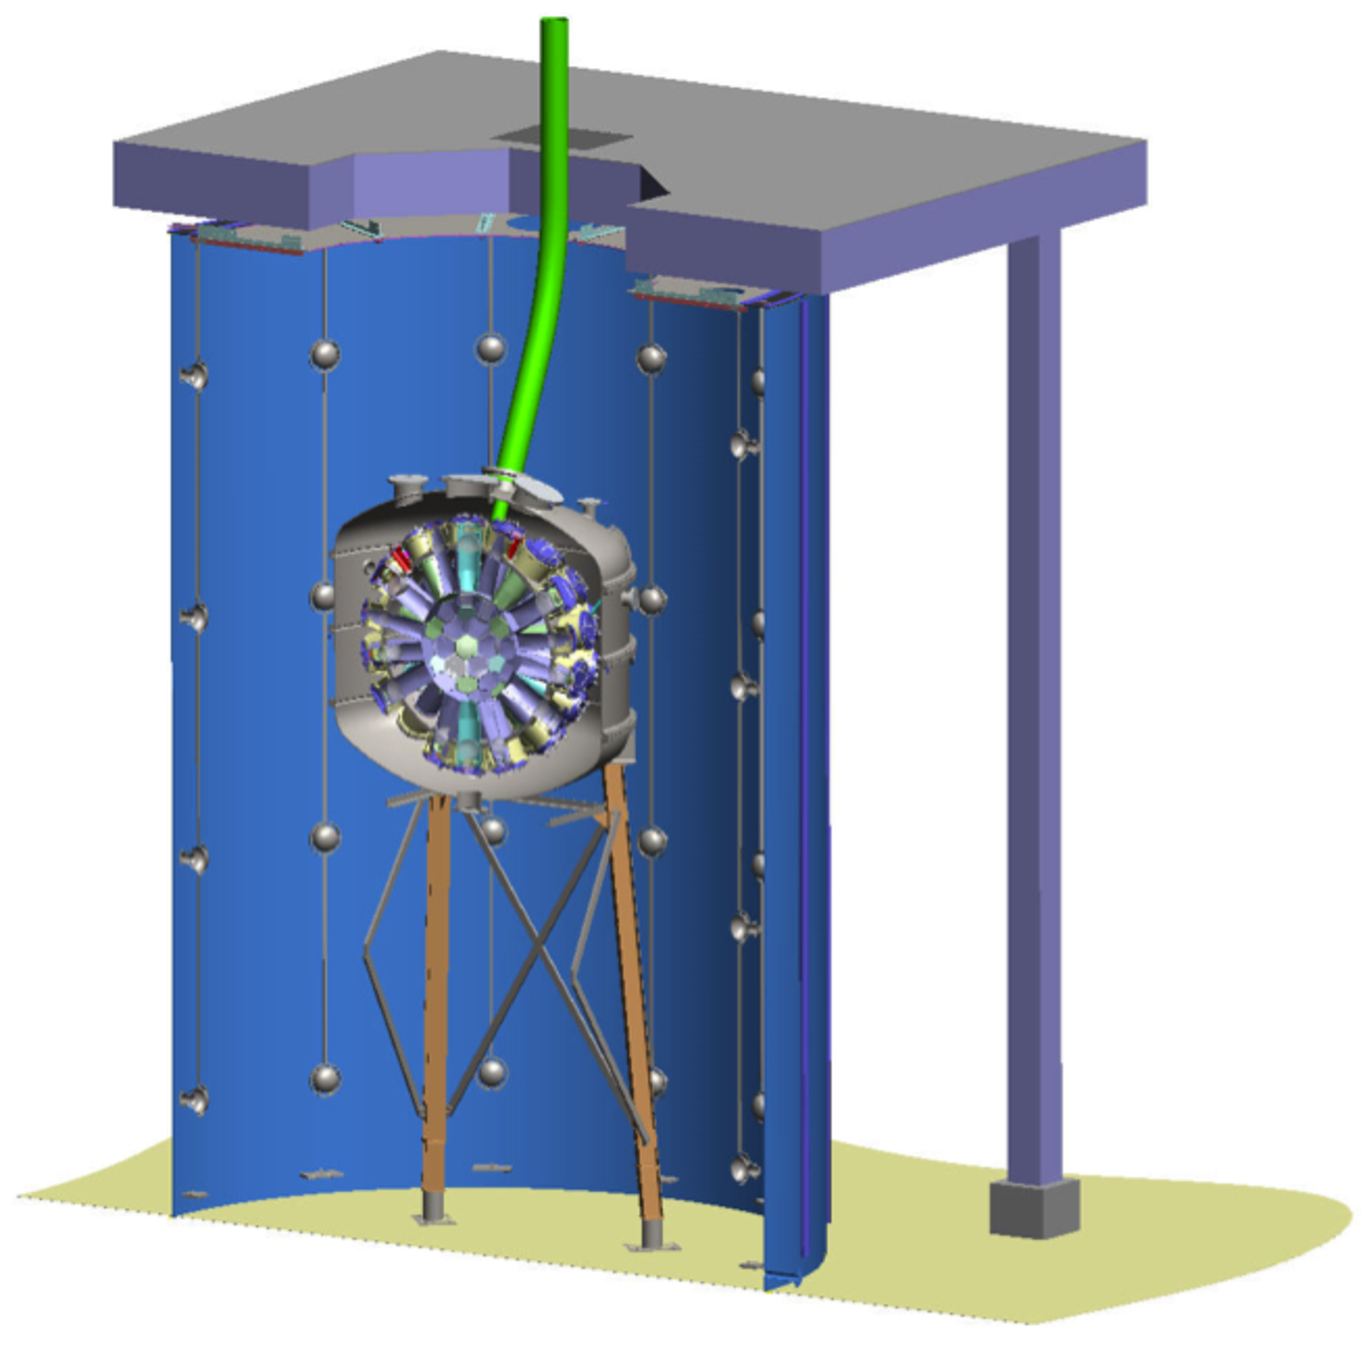
\includegraphics[width=3.5in]{graphics/miniclean_overview_drawing.pdf}
\caption{Model of MiniCLEAN veto showing the shield tank, inner liquid argon detector, and veto PMTs.
\label{fig:veto_geom}}
\end{center}
\end{figure}

\subsection{PMTs, connectors, cables}
\label{sec:pmts}
%
Sixty-six Hamamatsu R1408 PMTs were made available from SNO for use in the
MiniCLEAN veto. These PMTs were qualified to find the optimum
operating voltage, single p.e. charge mean and width, and noise rate in
tests done for the Sudbury Neutrino Observatory
(SNO)~\cite{ref:sno_pmt_paper}.  Operating voltages were chosen for an
anode gain of 1$\times$10$^7$.  The 66 PMTs were re-tested for
MiniCLEAN to verify the single p.e. charges and noise rates, following
the SNO PMT testing analysis procedure.  In all cases except one
broken PMT the test results were consistent with the SNO measurements.
At the operating voltage a typical single p.e. pulse charge is 1~pC,
with pulse amplitude of approximately 10~mV and pulse full width of
10~ns.

The MiniCLEAN veto PMT testing comprised of the following.  The gain and
dark rates of the PMTs were measured as a function of bias voltage
in a PMT test stand at Los Alamos National Laboratory.  This testing used a CAEN
V1720 digitizer with the MiniCLEAN DAQ software, DCDAQ, for data
acquisition \cite{ref:gastler_thesis}. PMTs were conditioned at 2100~V
for 12 hours. Next, a single photoelectron gain measurement as a
function of bias voltage was made using a blue LED flashed at low
intensity, such that PMT occupancy was several percent. Final gain and
dark rate measurements were made at the PMT operating voltage in a
similar test stand at MIT. Finally 48 PMTs plus 5 spares were selected for
use in the veto. 

The selection criterion was chosen to minimize dark rate, and thereby
minimize the rate of false veto triggers (discussed in Section
\ref{sec:electronics_design}).  We required the rate of pulses with
amplitude $>$3~mV to be less than 3000~Hz in the absence of a light
source.  The 3~mV pulse amplitude corresponds to a threshold of
0.2-0.25~p.e. for the 53 selected PMTs.  This threshold is motivated
by the Monte Carlo study which determined that for an N-Hit threshold
of 0.25~p.e. and a coincidence level of N-Hit$\ge$3, the predicted
muon veto efficiency is 0.999.  The range of operating voltages of the
selected PMTs was 1800-2300~V.  PMTs were then grouped by 8, choosing
operating voltages within $\pm$15~V per group, in order to gain match
the PMTs that are multiplexed in the veto electronics.  The spread of
single p.e. charges at the 3~mV amplitude threshold within a
multiplexed group is at most $\pm$0.05 p.e.

The SNO PMT bases are fitted with custom, waterproof TNC-type jack
connectors which mate 75 Ohm RG59 cable to the PMTs. These custom
connectors were built by the MIT machine shop from the SNO-TRIUMF
design. An assembly drawing of the connector is shown in
Figure~\ref{fig:connectordrawing} along with a picture of one of those
built at MIT. The MIT-built SNO
connectors were prototyped, tested at voltage in air, and tested at
voltage in water before the full connector complement was machined.
After cable assembly, all of the machined connectors were tested in
a test stand at RHUL in water at voltage with PMTs attached. All of the
PMTs were tested in water at voltage with the MIT-built connector
sample. Several failures of cable connectors were observed in dry
tests. These experiences were used to modify the cable assembly
procedure after which no cable connectors or PMTs were found to fail
these wet tests.


The connection to the PMTs uses a custom cable, Belden part number YR29304 Rev 2. The cable is a
RG-59 coaxial cable and is the same cable used by SuperK and SNO.
The cable is flooded, has a waterproof jacket and is rated to 2.3~kV.

The SNO PMTs have waterproof base enclosures, consisting of a plastic
cylinder filled with gel. All of the PMTs were immersed in water and
operated at voltage for approximately 4 hours in a test stand at MIT
to look for base waterproofing or connector failures. However, this
test did not simulate the water pressure at the bottom of the veto
tank. To study this issue, a pressure vessel was assembled at MIT
Bates Research and Engineering Center. This pressure vessel was used to test the PMT bulbs, base
enclosures, connectors, and cables for waterproofness and structural
integrity at pressure equivalent to that at the bottom of the veto.
Testing all of the PMTs at atmospheric pressure was successful and a
random subset of 10\% of the PMTs tested at 4 atm for several weeks (a
factor of 2 above the maximum pressure in the MiniCLEAN veto tank)
found no failures. Therefore we concluded that further encapsulation
of the SNO waterproof base enclosure was not necessary.

\begin{figure}[ht]
\begin{center}
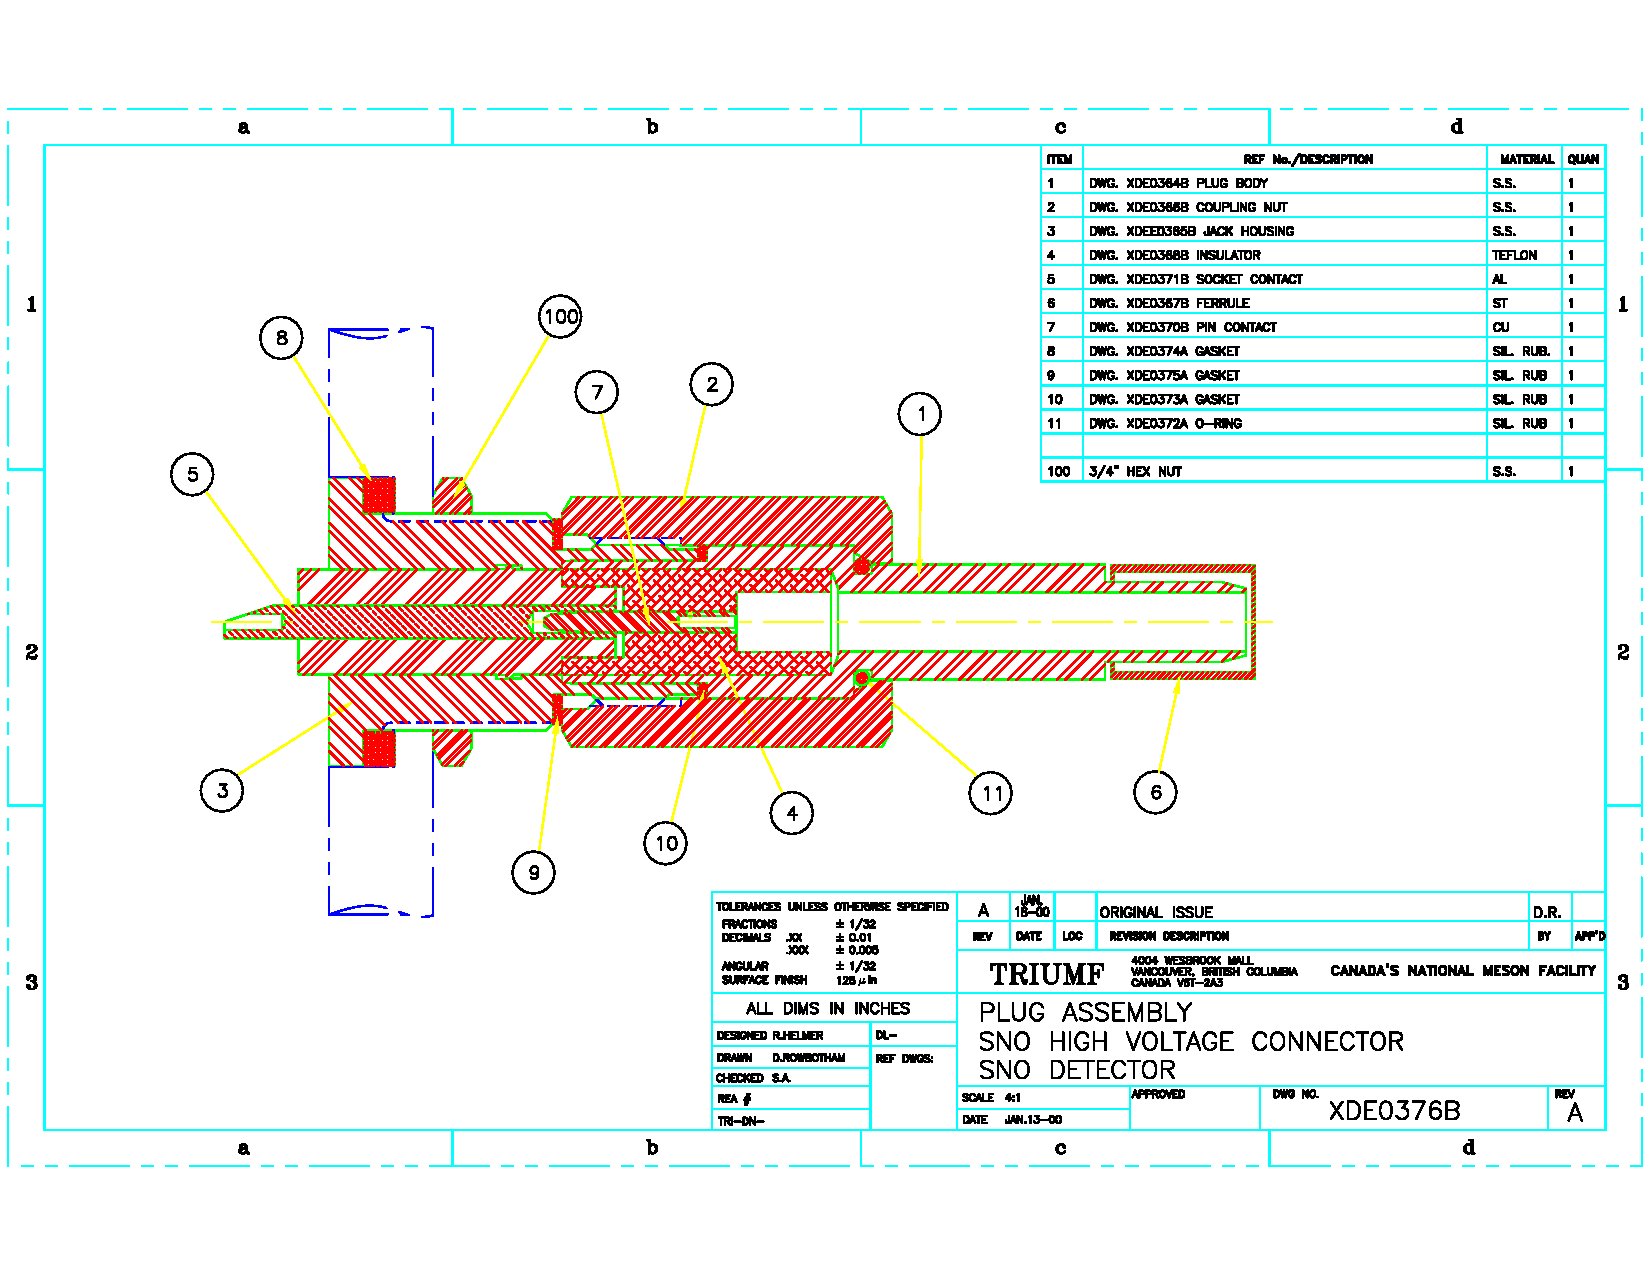
\includegraphics[width=2.75in]{graphics/snoConnectorDrawings.pdf}
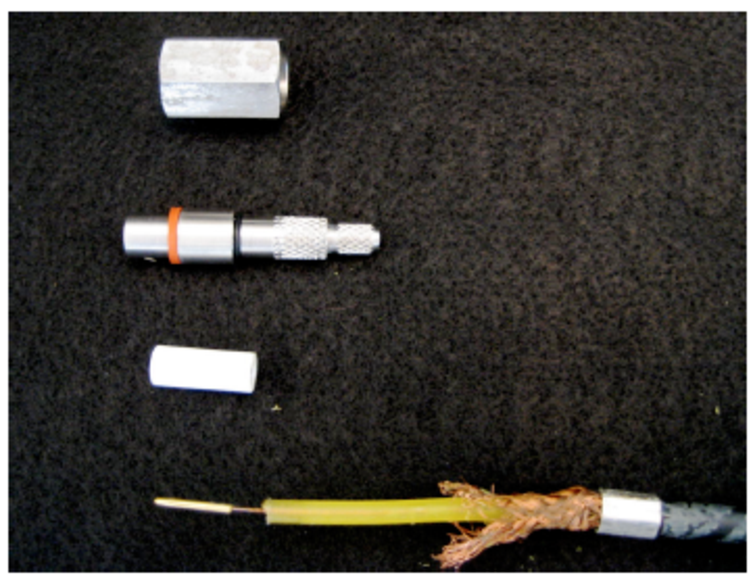
\includegraphics[width=2.75in]{graphics/connectorpic.pdf}
\caption{Left: TRIUMF connector assembly drawing. Items 1,2,4,6,7,10, and 11 were built or purchased to mate RG59 cable to the existing R1408 PMT jacks. Right: As-built TRIUMF connector for mating cable to the R1408 jack. From top to bottom is shown the coupling nut, the plug body into which the cable is inserted, the teflon insulator which is also inserted into the plug body, and the pin with a stripped cable.
\label{fig:connectordrawing}}
\end{center}
\end{figure}


\subsection{Mechanical hardware}
%
The PMT support structures attach the PMTs to poles or
``strings'' which attach to the veto tank lid. These were built at
MIT Bates Research and Engineering Center. 
%Drawings of the 316L stainless steel mount and string are shown in Figures~\ref{fig:vetopmtmount} and \ref{fig:vetopmtstring}, with pictures of the hardware in Figure~\ref{fig:vetopmtmountpic}. 
The 316L stainless steel mount and string are shown in
Figure~\ref{fig:vetopmtmountpic}. The
Buna-N rubber pads contacting the base enclosure and bulb accommodate
the variations in dimensions across the set of PMTs. The base
enclosures' and bulbs' diameters were measured to vary between 3.00
and 3.34 inches and between 7.91 and 8.02 inches. The rubber mounting
pads were all fit by hand to each PMT at Bates before shipment to
SNOLAB and tested with a load of twice the buoyant force (maximum
8~lbs/PMT) to try to dislodge the PMT from the mount. This procedure
will be repeated during assembly to verify the mechanical stability of
each veto PMT in its mount. These tests were done with both wet and dry
rubber pads. A complete assembly test of one string, consisting of
four PMTs and associated hardware, dry, was done Bates (shown in Figure~\ref{fig:vetopmtmountpic}, right).

\begin{figure}[ht]
\begin{center}
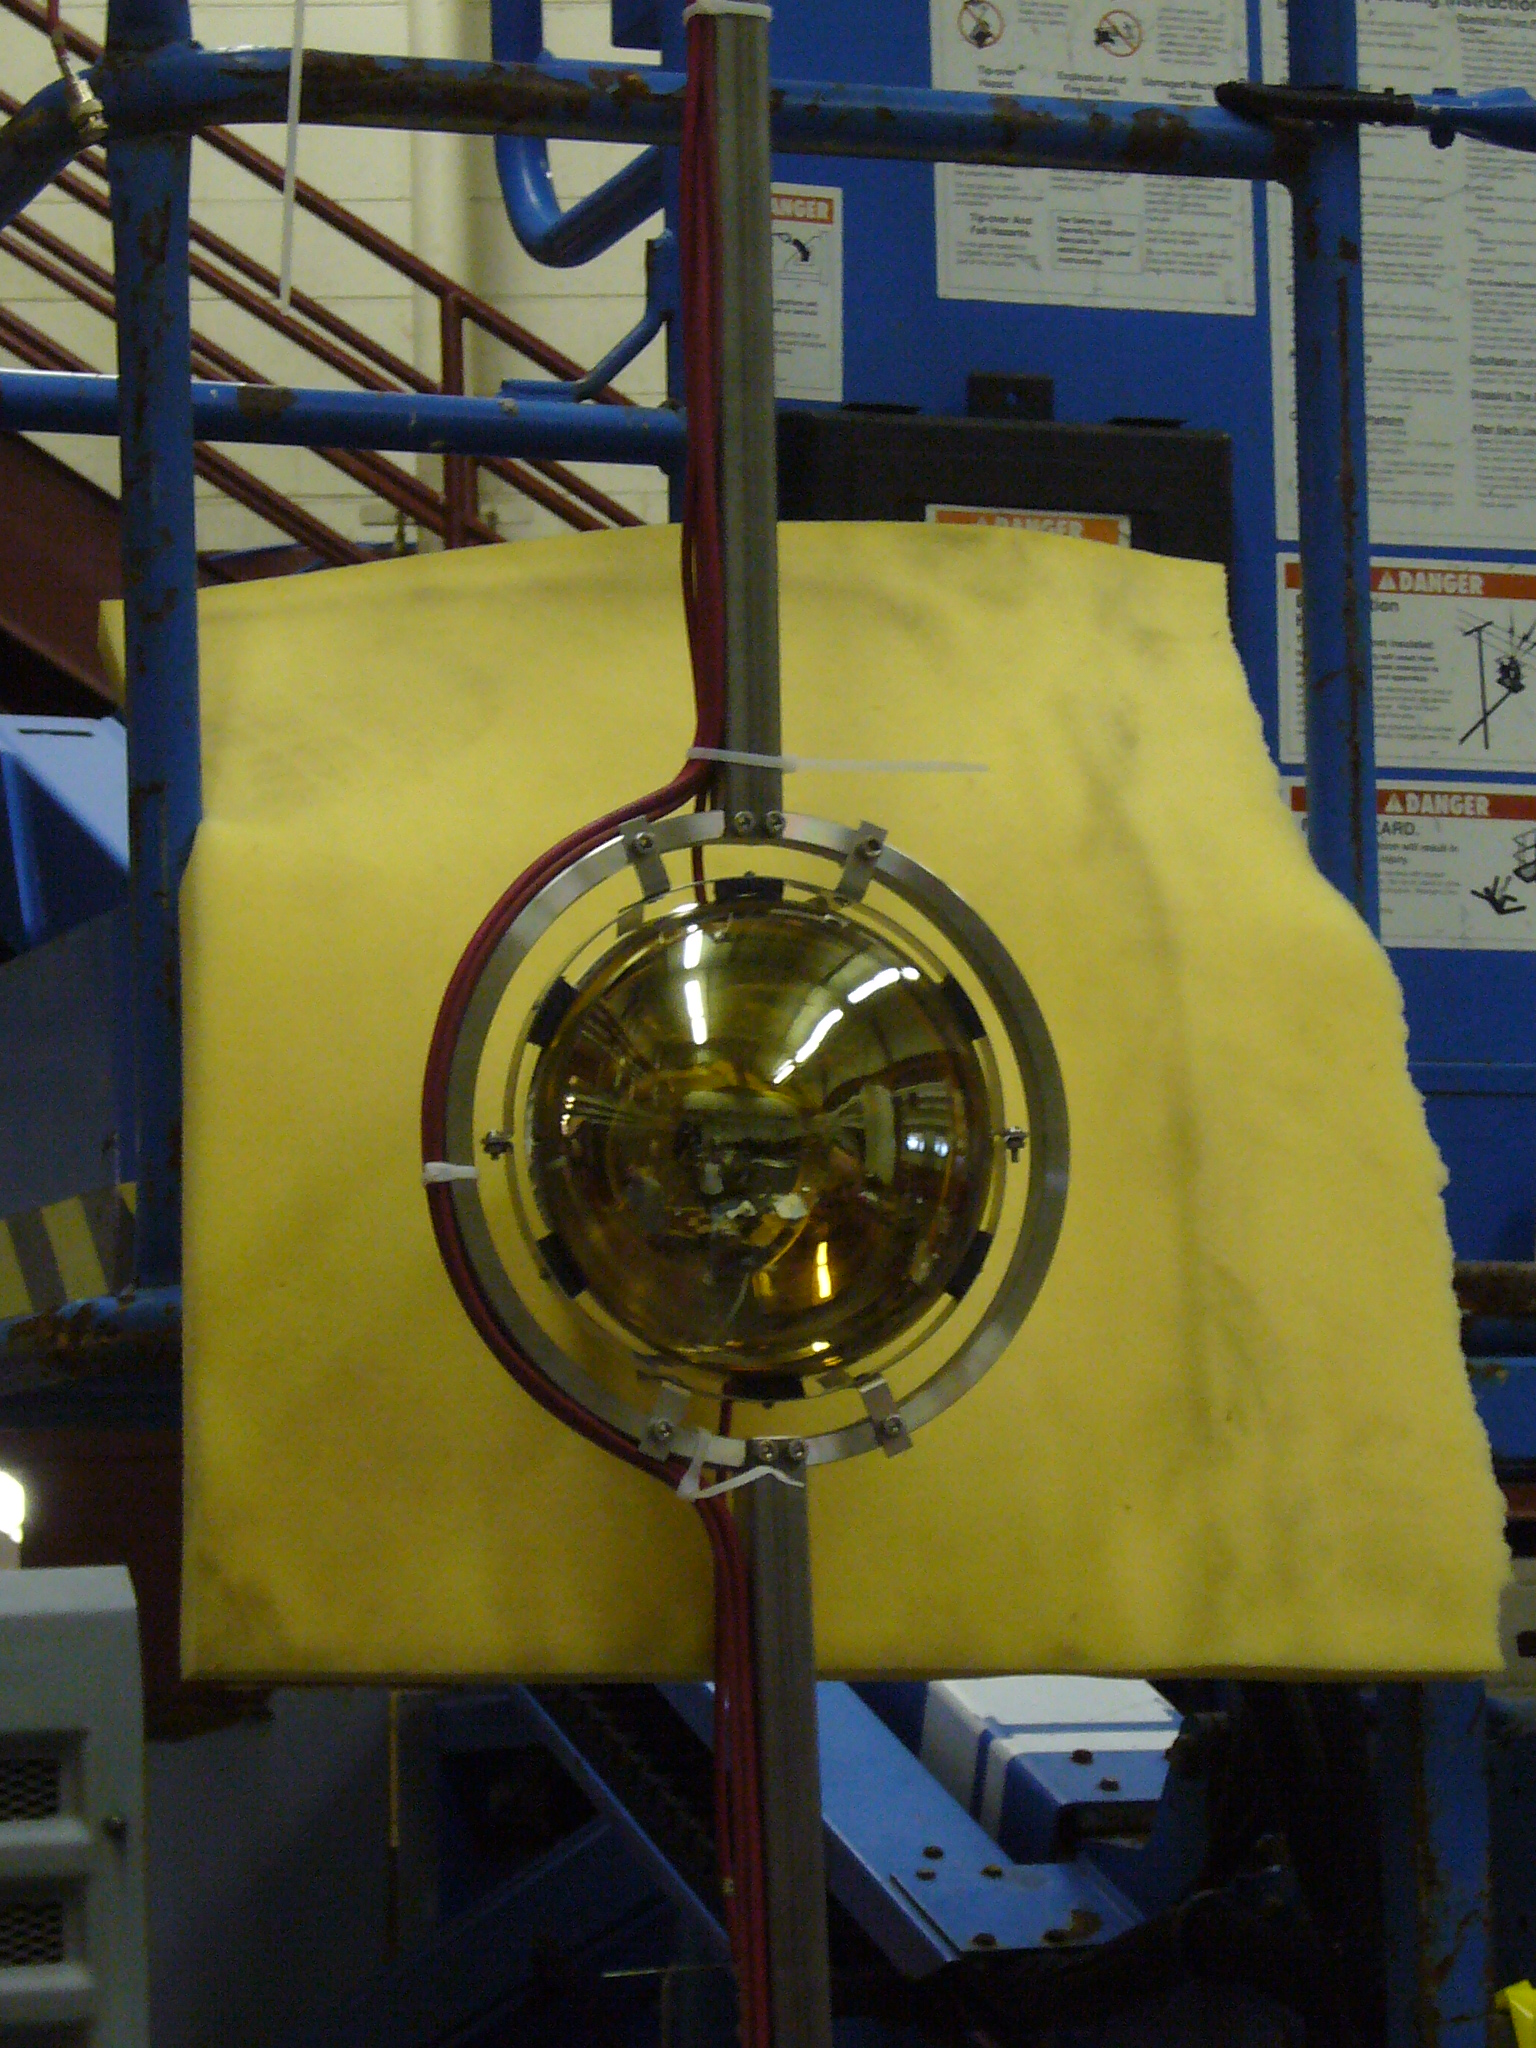
\includegraphics[width=2.in]{graphics/singlepmtmounted1.JPG}
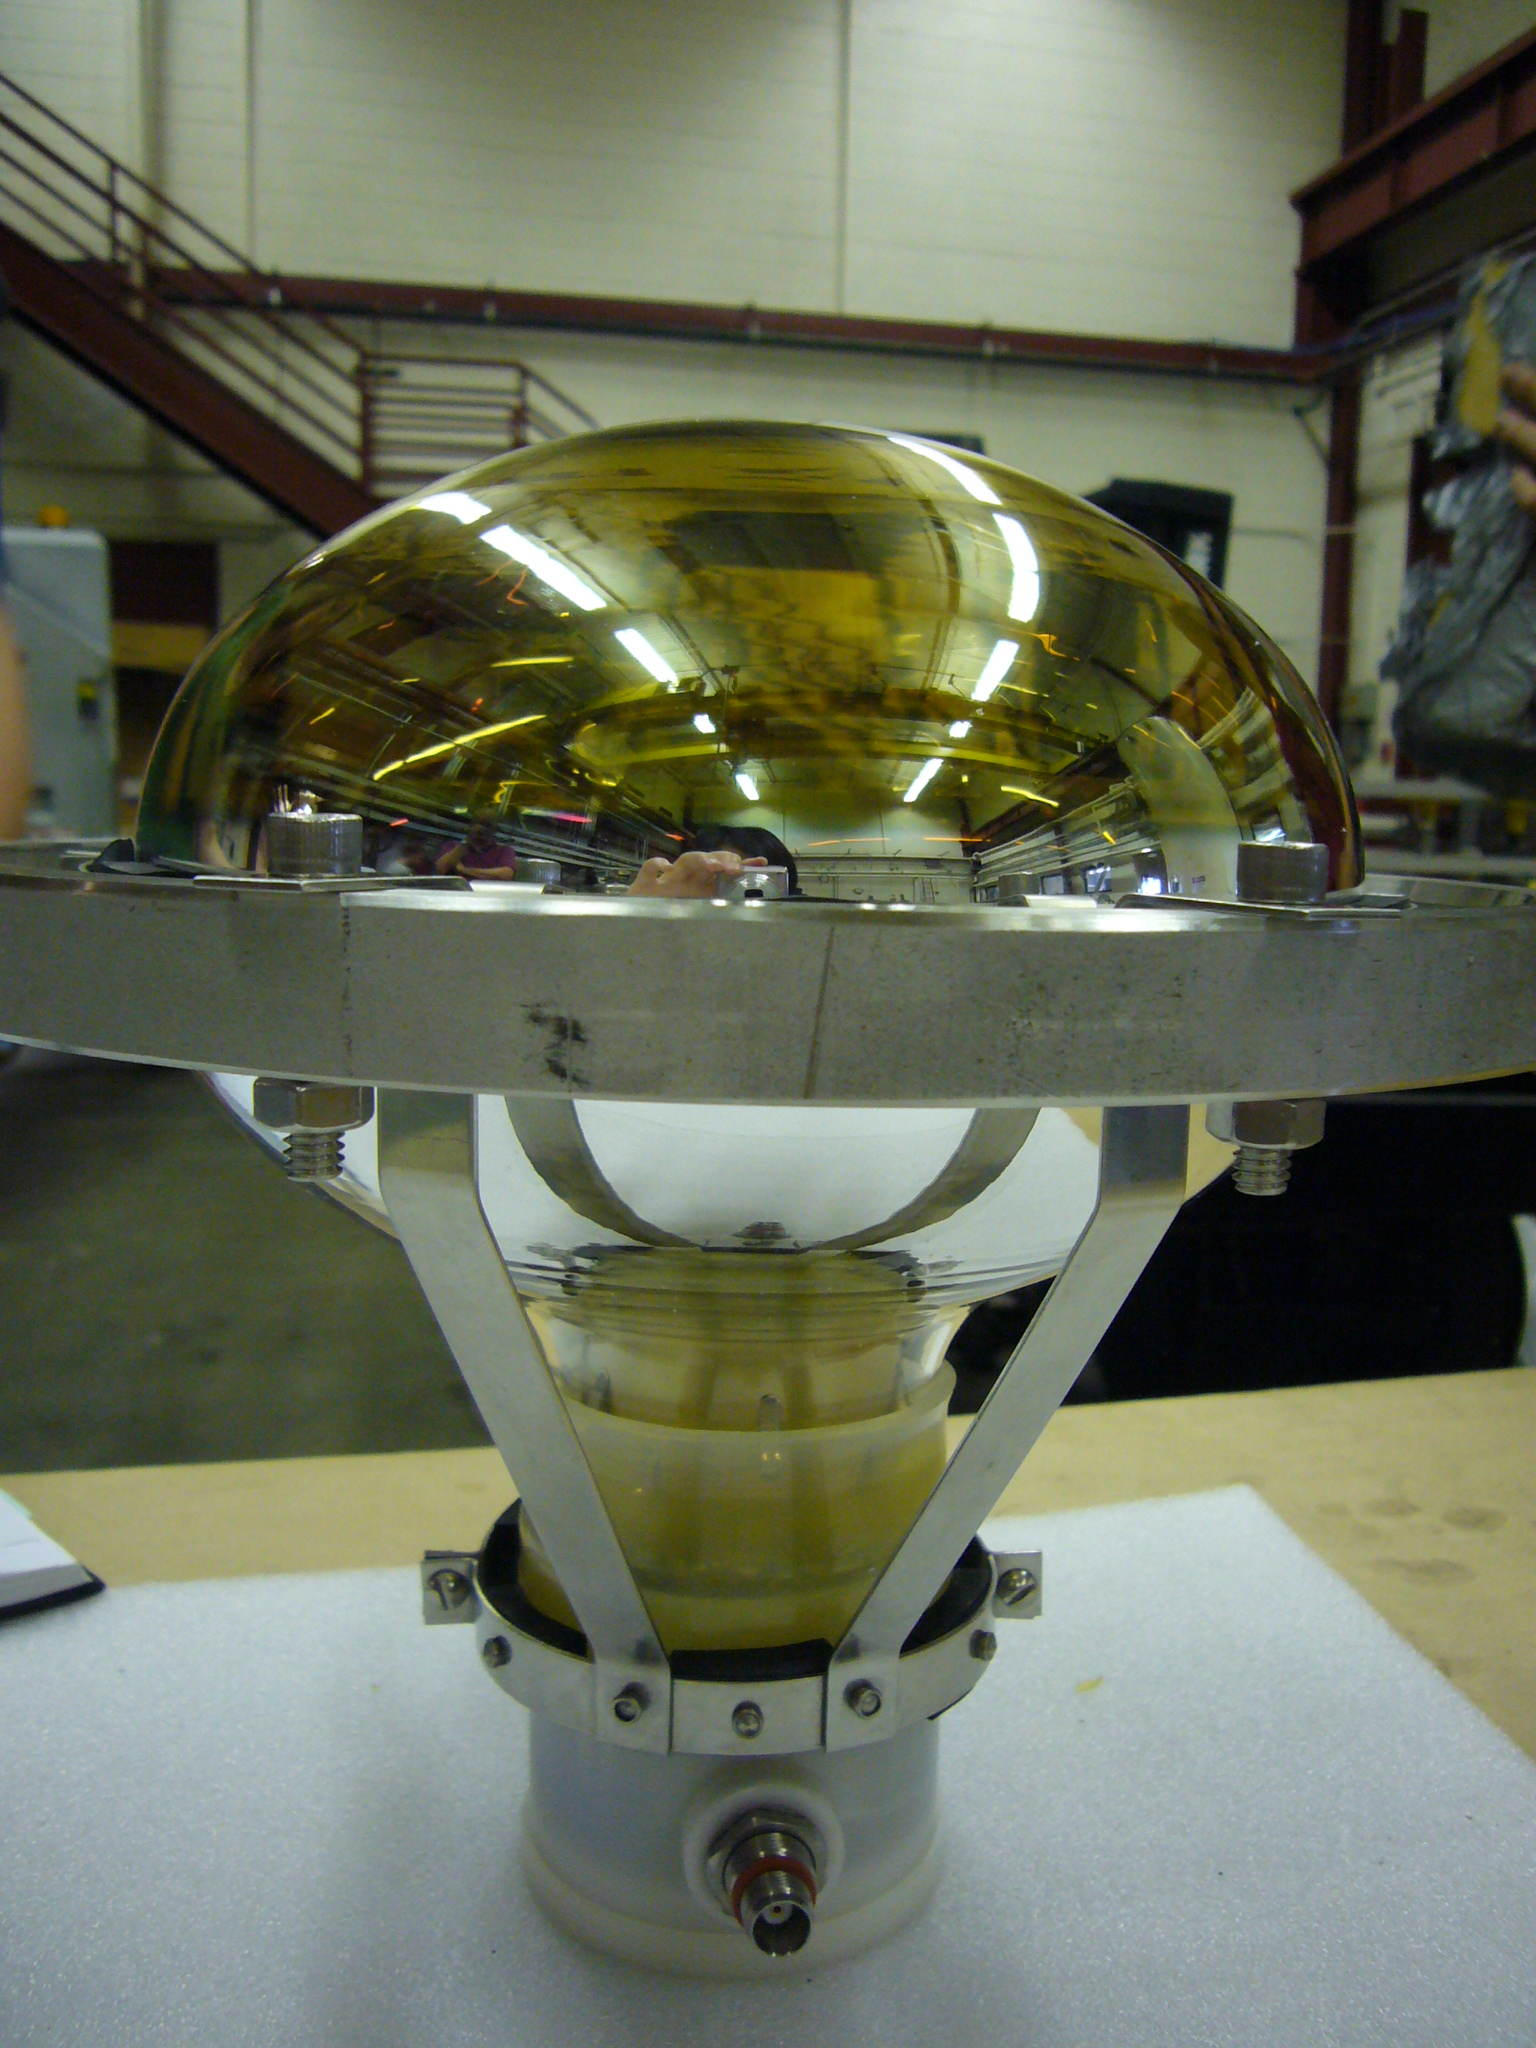
\includegraphics[width=1.9in]{graphics/singlepmtmounted2.JPG}
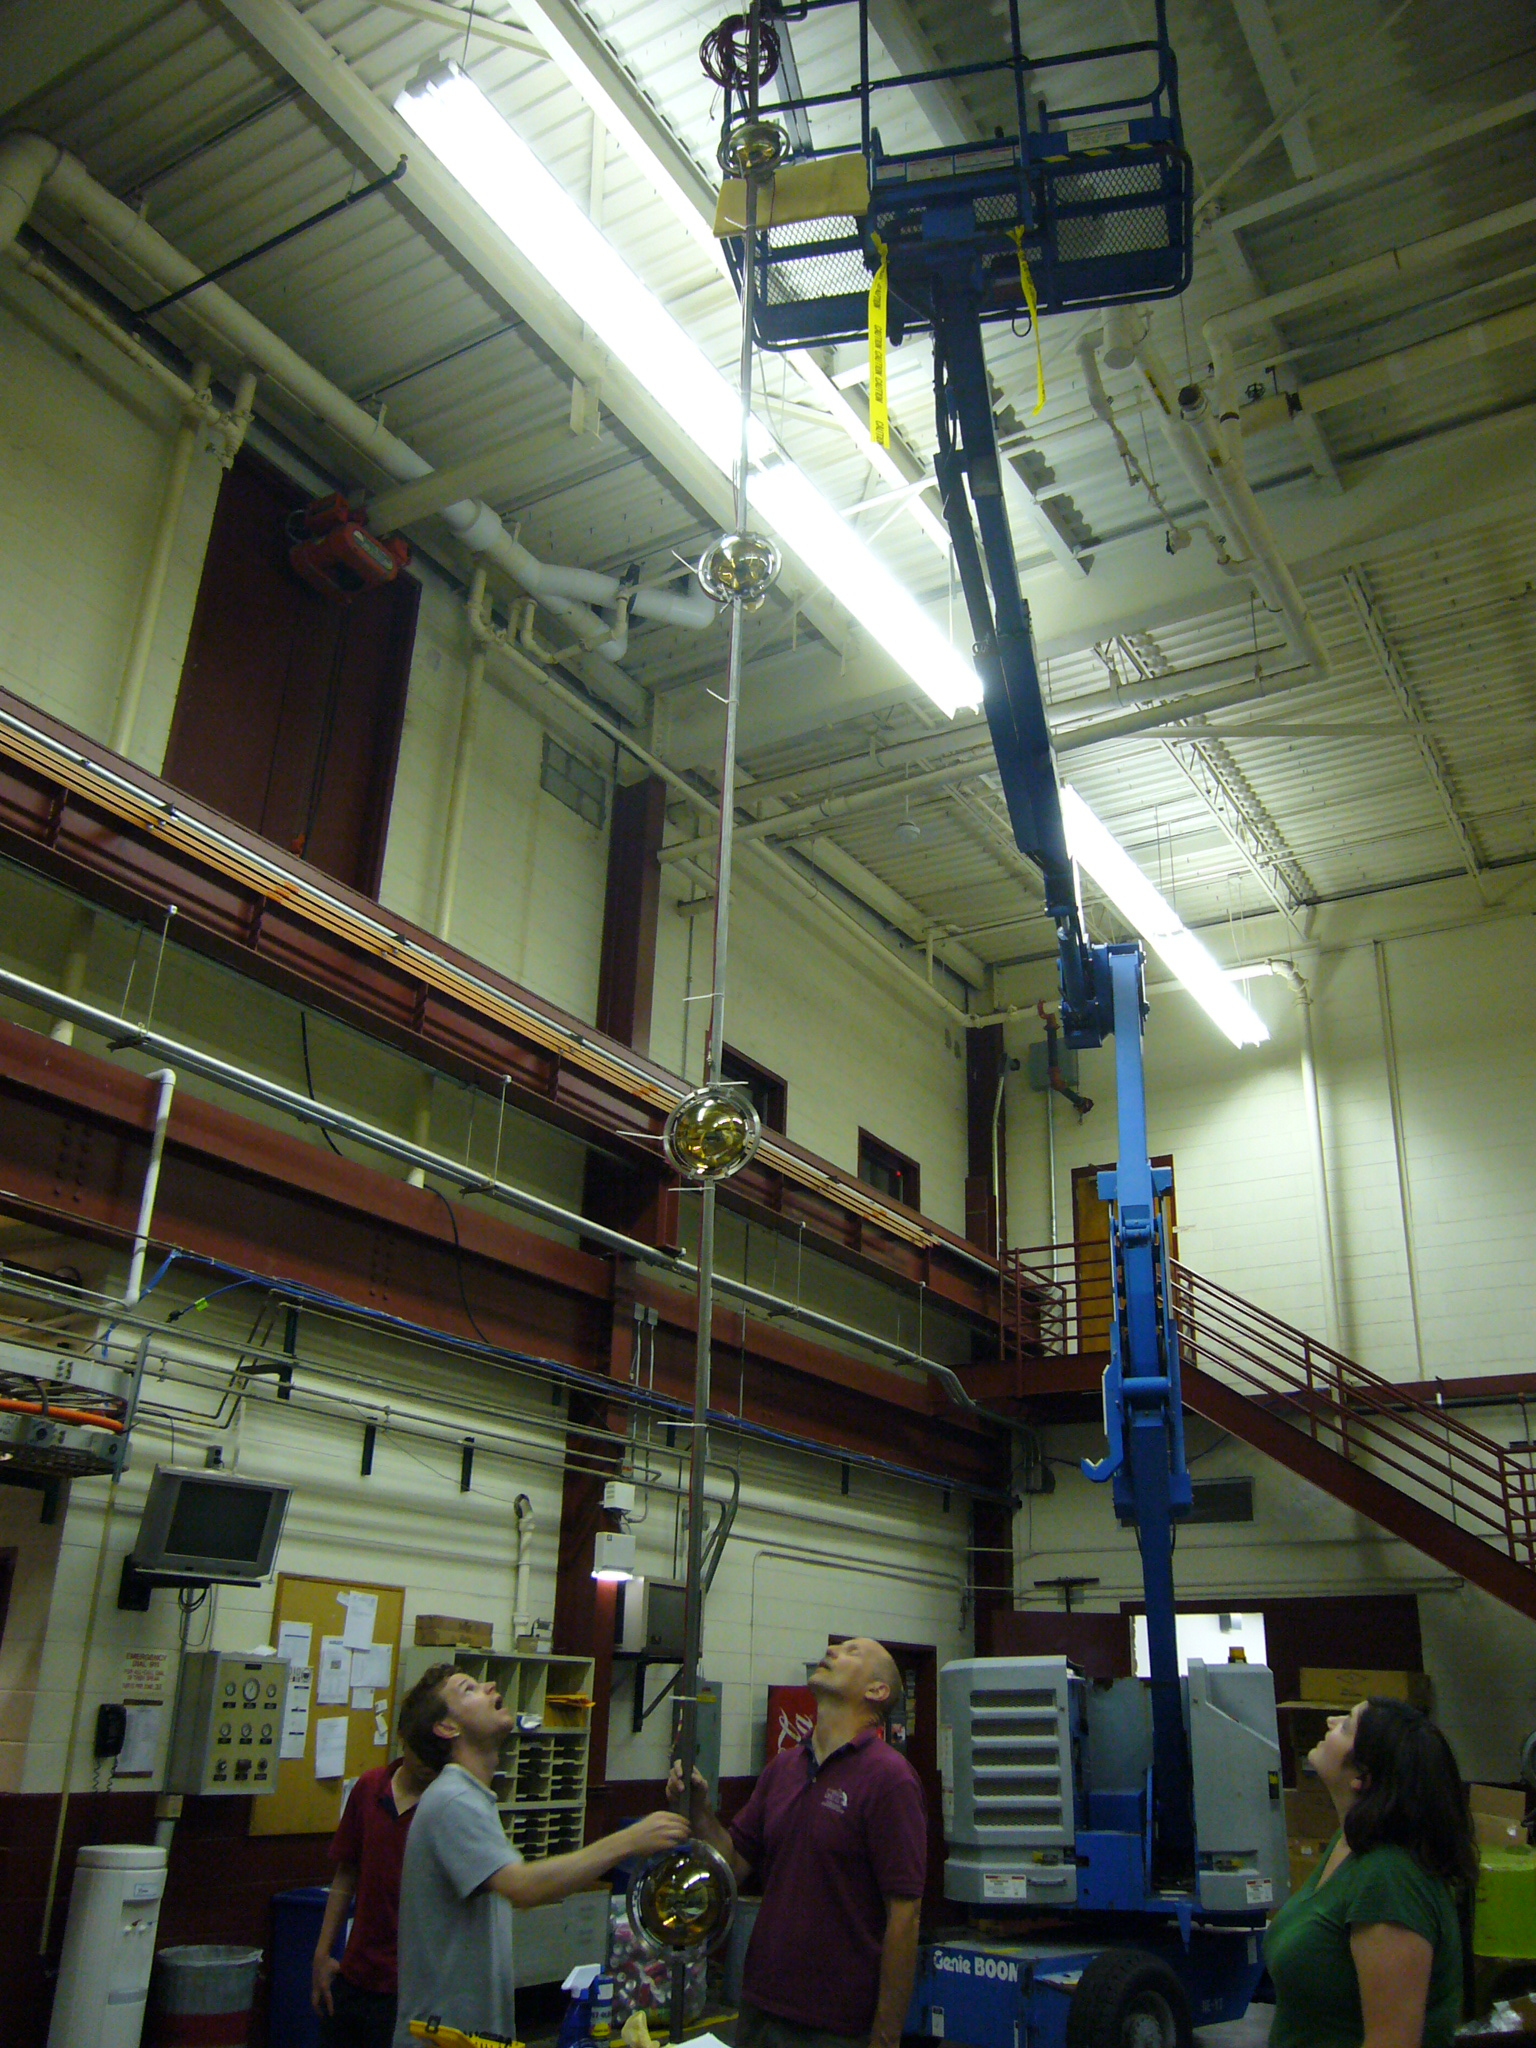
\includegraphics[width=1.9in]{graphics/pmtstring.JPG}
\caption{Veto PMT shown in mounting hardware (left, center), and assembled into a 4-PMT string (right).
\label{fig:vetopmtmountpic}}
\end{center}
\end{figure}


\section{Electronics design of the MiniCLEAN veto subsystem}
\label{sec:electronics_design}
%
The electronic components of the veto subsystem are the PMT high
voltage supply, the PMT signal electronics, and the data acquisition
electronics. A schematic of the system is shown in
Figure~\ref{fig:block_diagram}.

The veto PMT signal electronics consist of 6 amplifier discriminator
boards, which each service 8 PMTs, and 7 summer boards designed and
built by MIT Bates Research and Engineering Center.  To supply the
bias voltage to the 48 veto PMTs, 6 channels of a 12-channel card of
the MiniCLEAN liquid argon detector PMT high voltage supply (LeCroy
1461 VISyN) are used. The voltage divider circuits that distribute
power from each of 6 HV channels to 8 PMTs are part of the amplifier
discriminator board described in Section~\ref{sec:Amp-Disc}.  To
digitize the veto PMT signals, 7 channels on one 8-channel CAEN V1720
digitizer card of the MiniCLEAN DAQ system are used.  A key feature of
the veto system electronics is multiplexing the signals from 48 veto
PMTs down to 6 digitizer channels.  The veto signal multiplexing
electronics are part of the summer board described
Section~\ref{sec:Sum}. The MiniCLEAN CAEN DAQ is described in detail
in~\cite{ref:gastler_thesis}.

The rationale for multiplexing the veto PMT signals is the relatively
high cost-per-channel of the digitizing electronics.  The veto
electronics time multiplex 8 PMT channels onto a single digitizer
channel. For the veto, 7 digitizer channels were available. We use
6 of them to digitize the time-mulitplexed response from the
PMTs and use the 7th to digitize the instantaneous N-Hit sum signal
across the veto channels.  This approach minimizes the information
loss from multiplexing since the instantaneous N-Hit sum signal can be
used to verify that there are no hits in the veto volume when a
candidate WIMP dark matter event is recorded, and the time-multiplexed
signals can be used to study muon signals in the veto in greater
detail to validate the cosmogenic background prediction from simulations.

The instantaneous N-Hit sum signal across the veto is sent to a
discriminator module, which generates a NIM output pulse.  The N-Hit
threshold for the veto trigger is determined by the discriminator
level setting.  The NIM output pulse is sent to the MiniCLEAN trigger
module to form the veto trigger signal.  This module is described in
detail in~\cite{ref:gastler_thesis}.  Briefly, it accepts analog
trigger signals from a variety of inputs, constructs a trigger mask to
record which triggers are active at each timestamp, and fans the master
trigger signal out to the digitizer boards to cause acquisition of a
waveform from all channels, forming an event.  Given the low expected
rate of muons traversing the veto, the veto trigger signal is used to
cause data acquisition across the full detector rather than to prevent
the DAQ from recording data when a veto signal is present.  The veto
trigger level is adjustable, with a threshold voltage set in hardware.
The plan for operations is to set this level corresponding to
N-Hit$\ge$3.  Given the N-Hit threshold per PMT of 0.25 p.e., the
maximum allowed veto PMT noise rates at this threshold (3000 Hz), and
50 ns coincidence window, the expected rate of false coincidences at
this level is $<$7$\times$10$^{-5}$~Hz.  Using the average measured
noise rate of the selected PMTs (1800 Hz), this false coincidence rate
drops by a factor of 5, giving an expected signal-to-noise ratio in
the veto trigger of approximately 10-to-1.


\begin{figure}[ht]
\begin{center}
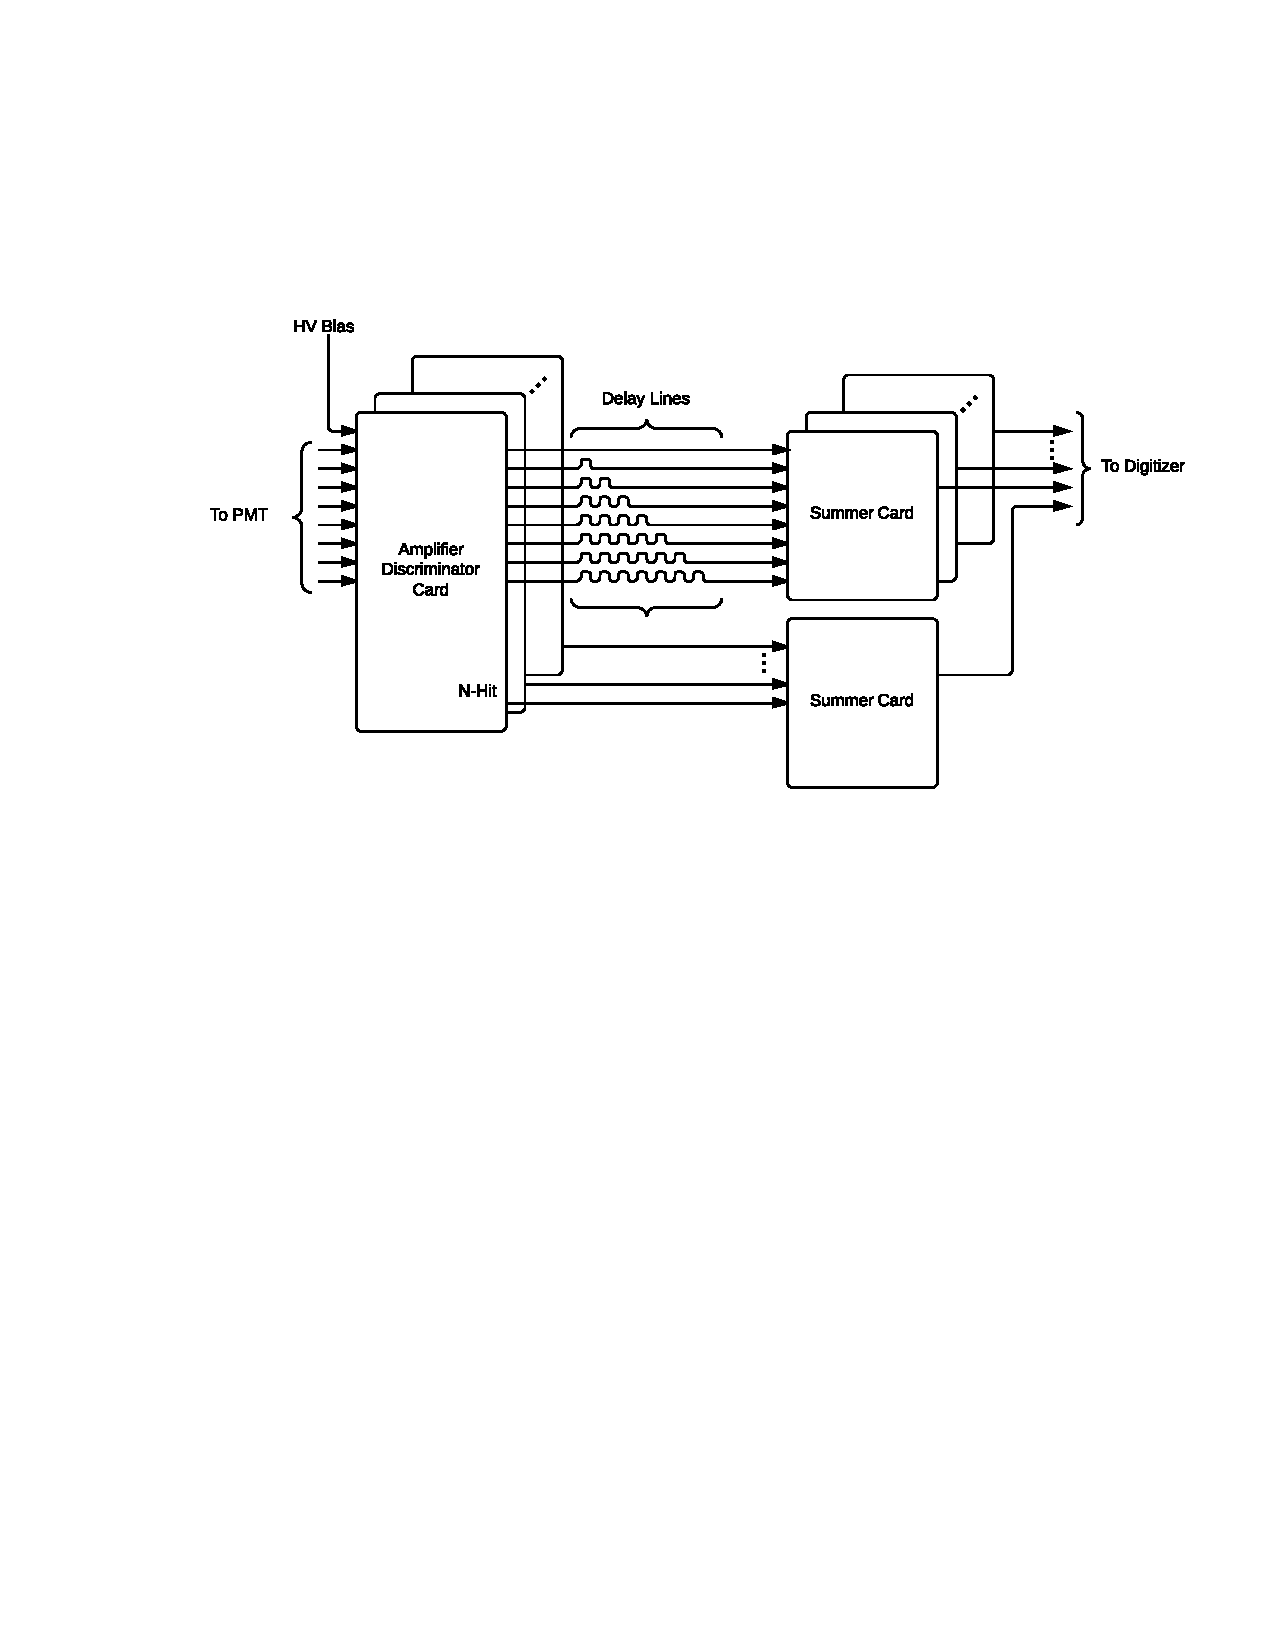
\includegraphics[width=5in, keepaspectratio=true, trim=1.25in 5.75in 0.5in 2in, clip=true]{graphics/block.pdf}
\caption{Block Diagram of MiniCLEAN Veto Electronics
\label{fig:block_diagram}}
\end{center}
\end{figure}

\subsection{Amplifier discriminator board}
\label{sec:Amp-Disc}
%
The amplifier discriminator board is the front-end electronics board.
The board provides high voltage distribution to the PMTs, signal
amplification, and signal discrimination for the N-Hit sum. The
board-wide PMT bias voltage is fed from a channel on a high voltage card
to an input SHV connector on the board. A voltage divider circuit distributes the bias to
each of the 8 PMT connections on the amplifier discriminator board.
PMTs with a similar operating voltages and single p.e. charges are
grouped onto a single amplifier discriminator board, as described in
Section~\ref{sec:pmts}, such that a single bias voltage can be used for
8 PMTs. Each PMT capacitively couples the signal onto the bias voltage
line, and each channel has an amplifier input capacitively coupled to
its PMT bias line. The schematic for the PMT bias scheme, along with
two channels of the amplifier discriminator, is shown in
Figure~\ref{fig:ampdiscsch}.

\begin{figure}[ht]
\begin{center}
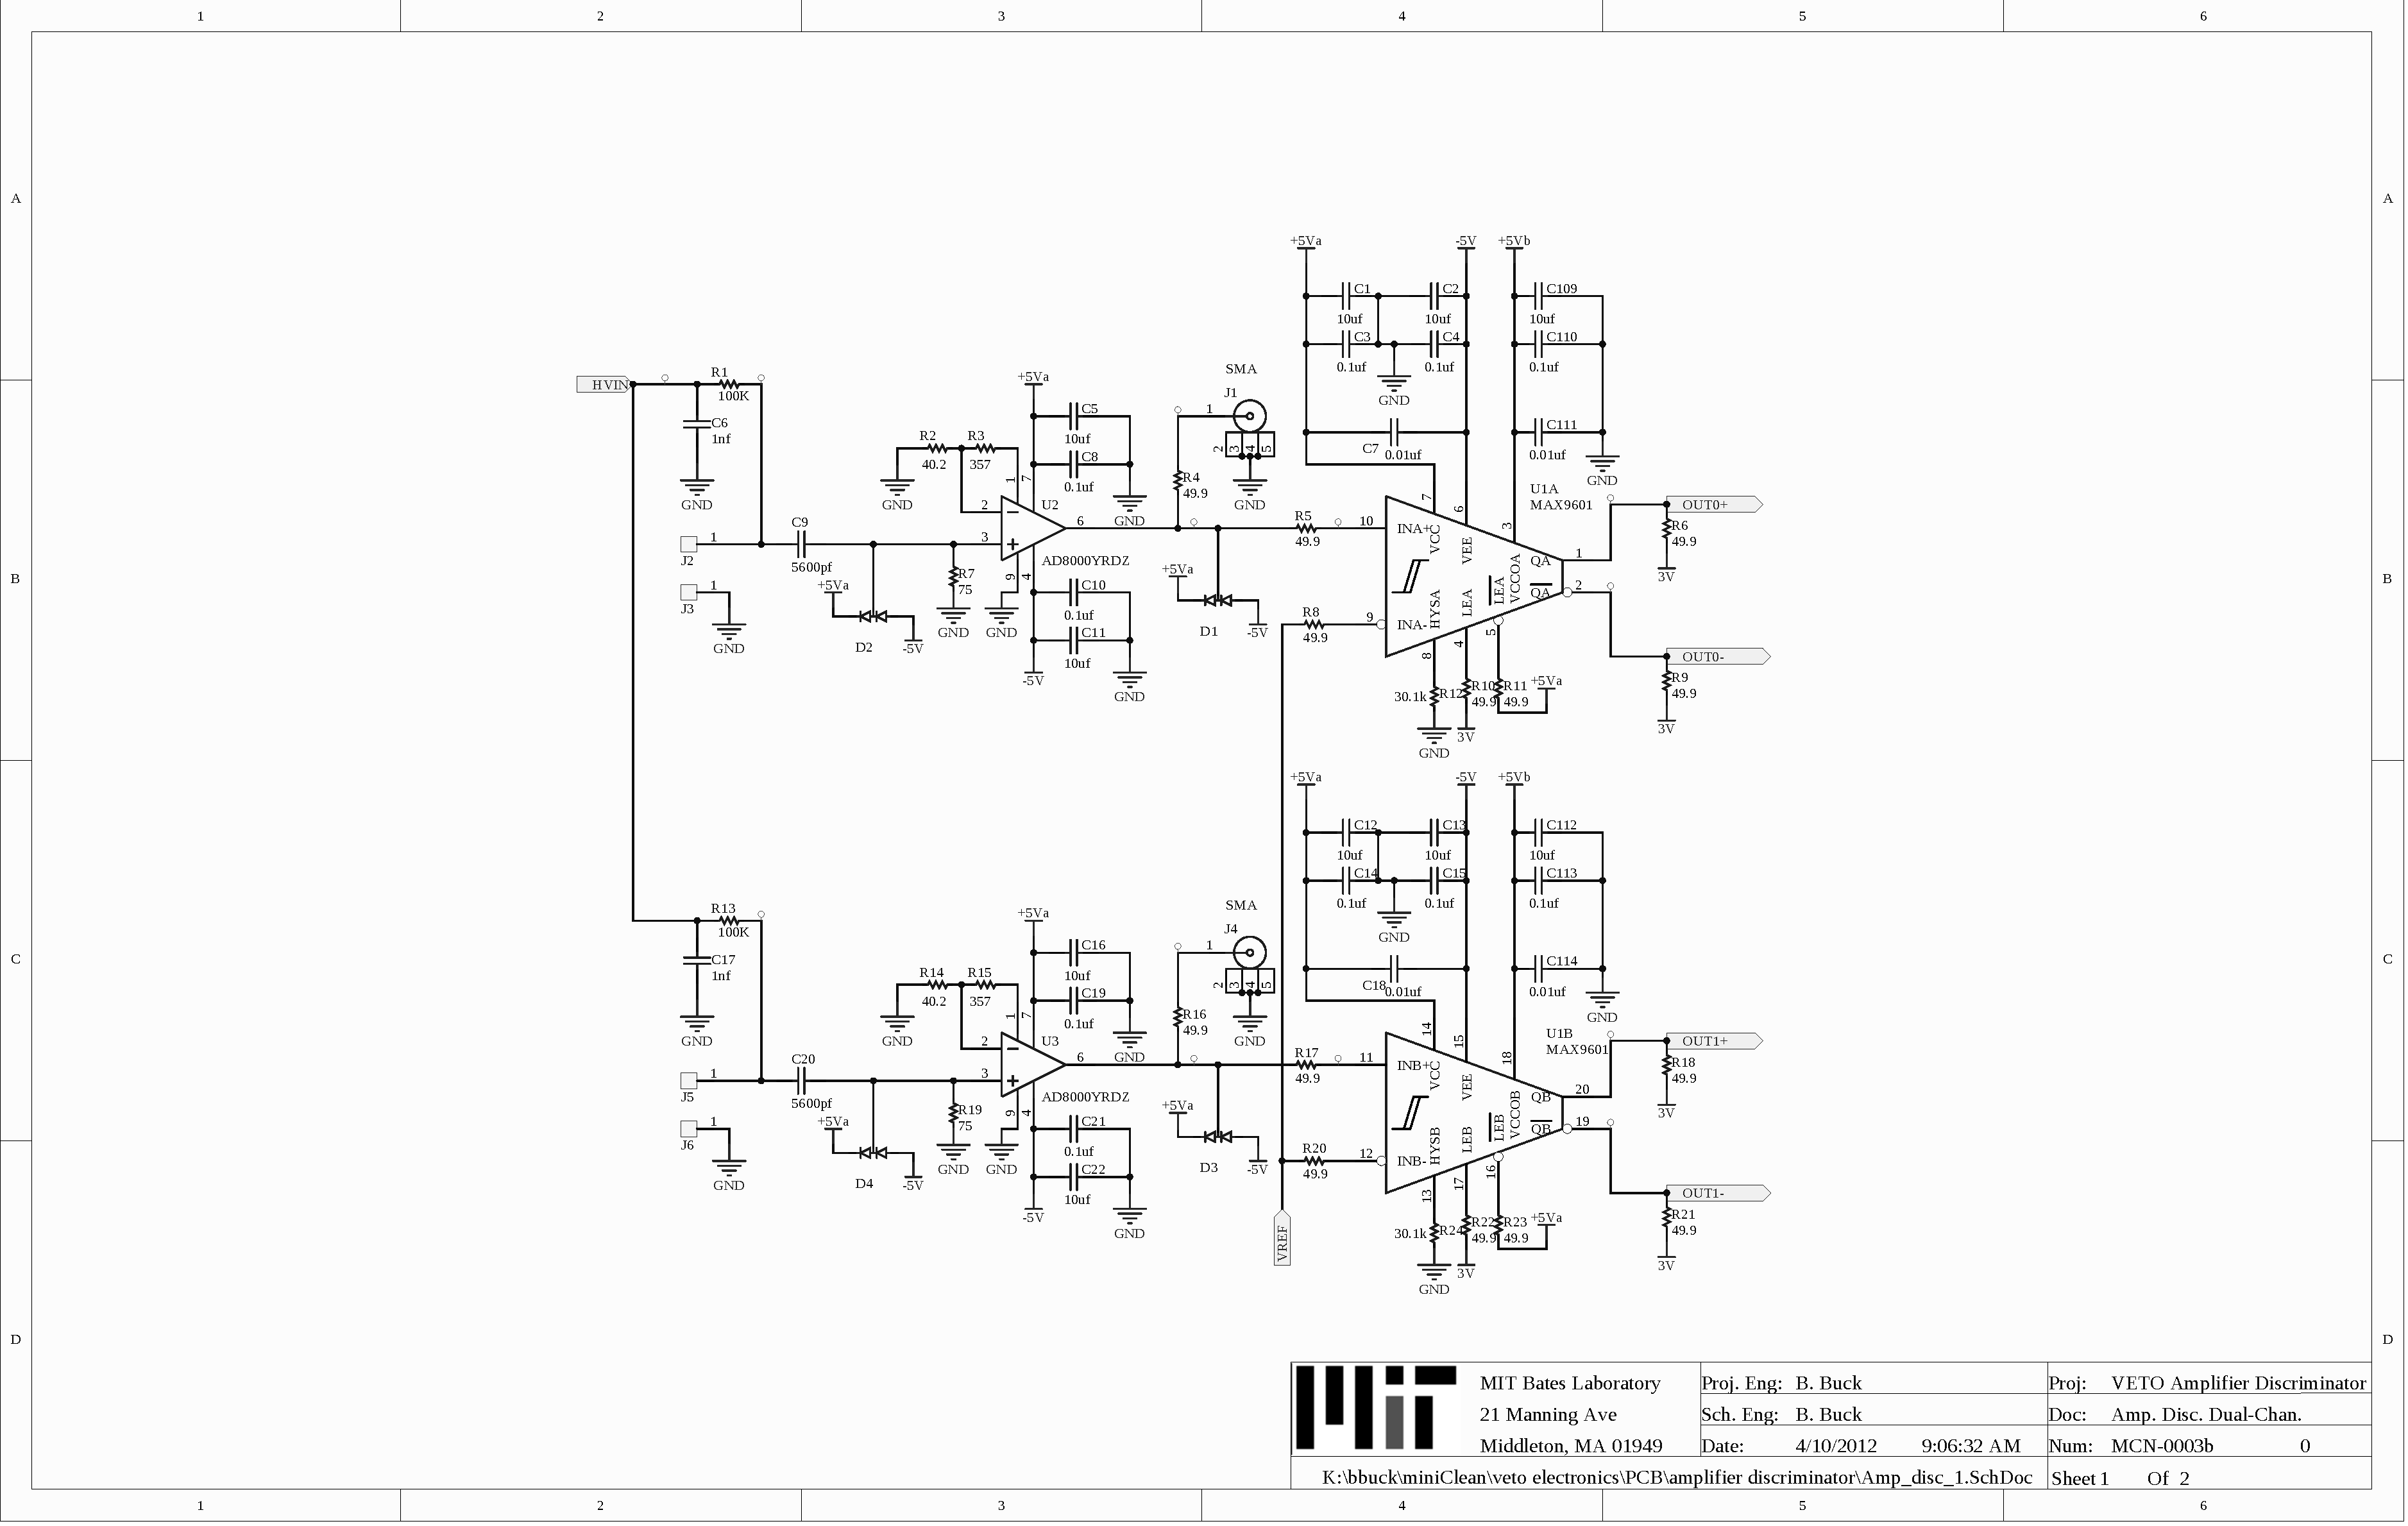
\includegraphics[width=5.5in, keepaspectratio=true, trim=4.54in 2.12in 4.54in 2.12in, clip=true]{graphics/veto_sch.pdf}
\caption{Two channels of the amplifier discriminator board. J2 and J5 make the signal connections to the PMTs. J1 and J4 make the connections to the delay lines. U2 and U3 are the amplifiers, U1 is the two channel comparator.
\label{fig:ampdiscsch}}
\end{center}
\end{figure}

The HV bias components are surface mount types. Because of the aspect
ratio of the width and length of some of the components, they had to
be raised slightly off of the board during the soldering process to
ensure that flux could be cleaned from underneath the components. In
addition, the HV components were potted with corona dope after
assembly.

To handle the relatively low target discriminator threshold of 3~mV,
and the amplitude decrease associated with time multiplexing method we
use, we amplify the signal pulses by a factor of 10.  A high
bandwidth current feedback amplifier (CFA) provides the large gain and
bandwidth needed to amplify the pulses by a factor of 10 in a single
stage. We use the Analog Devices AD8000 as the CFA in both
the summer board and in the amplifier discriminator board. The amplified
pulses are fed out to the delay lines
and to on-board comparators for discrimination.  Due to the high gain
requirements, and the variations between the amplifiers, all of the parts
installed were tested beforehand and binned into parts with a similar
DC offset.  During board assembly, care was taken to ensure that all
of the amplifiers installed on a single board had a DC offset which
varied by no more than 10\%.

The comparator compares each channel with a programmable threshold
voltage, common to all 8 channels on each board. The output of the
comparator is a fast differential PECL pulse. The comparator outputs
from the 8 channels on each board are summed with a differential
amplifier and output using a transformer as a single ended signal to
produce the N-Hit sum for each board.

The amplifier discriminator board has local linear power regulation.
Each board has two +5~V supplies, one -5~V supply, and one +3~V
supply.  The CFA runs on the +5~V and -5~V supplies. The comparator
runs on the second +5~V supply and the +3~V supply (necessary for PECL
output).  The two +5~V supplies isolate the output supply for the
comparator in order to reduce cross talk. The regulators are fed by a
common bipolar supply and ground, nominally at $\pm$9~V. The nominal
values for current draw are 500~mA on the positive rail and 250~mA on
the negative rail.

The board is constructed with 4 copper layers and standard FR4
substrate material, with 0.062 inch thickness. It is mounted on a piece
of FR4 to protect HV nets on the bottom of the board from arcing and
to fit it into a 6U VME style crate. 9 SHV connectors are mounted on
a front panel connected to the FR4 and provide the HV bias input and
eight PMT connections. These PMT connections attach on the left side
of the board with short insulated wire pig-tails. On the right
side of the board 9 SMA connectors are board mounted. The SMA
connectors provide the 8 signal outputs to the delay lines and the
N-Hit sum signal. A photo of the amplifier discriminator
board is shown in Figure~\ref{fig:boards}.

\subsection{Delay lines}
\label{sec:Delay}
%
Delay lines are used to time multiplex the signals.  Typical PMT
signal pulses are $<$15~ns long, as discussed in
Section~\ref{sec:subsystem_design}.  We use 50~ns as the increment
of delay in the time multiplexing in order to minimize pile-up in time
of signals from multiple PMTs.  To handle 8 channels, the maximum
delay required is 350~ns, which is beyond the capability of current
active delay components.  Therefore we use passive cables to delay the signals.

The delay lines connect from the amplifier discriminator boards to the
summer boards. They are designed to delay the signals between 0~ns
(for the first PMT channel of each amplifier discriminator board) and
350~ns (for the eighth channel), in steps of 50~ns.  After delay, the
signals from each amplifier discriminator board are summed together by
the associated summer board, which has the effect of time multiplexing
the signals.  

The delay lines are made of different lengths of Belden 9310 cable
fitted with male SMA connectors. The cable is chosen for its low
attenuation, slow signal propagation speed, and small bend radius.
There are 7 different lengths ranging form 32~ft to 224~ft, with every
32~ft corresponding to 50~ns of delay. The delay lines are coiled
inside a metal box with pig-tails to connect to the amplifier
discriminator boards and the summer boards. The metal box satisfies
fire protection regulations in the mine, as the Belden 9310 is not
plenum rated. There are two sets of each of the seven lengths in each
box.  One of the signals has a $\sim$0~ns delay and is connected from
the amplifier discriminator board to the summer board with a very short
jumper cable.

Figure~\ref{fig:multipulse} shows the time multiplexed output of 8
channels fed with a synchronous pulse of constant amplitude.  The
amplitude of the pulses decreases by approximately 30\% from the first
to the eighth delayed pulse.  This is due to the attenuation of the
longer delay line.  This amplitude decrease can be calibrated out in
the analysis of the multiplexed signals, using this synchronous
constant input pulse measurement.

Another complexity introduced by time multiplexing is the
increased probability of PMT noise pulses, such as from thermionic
emission or afterpulsing, piling up with PMT signal pulses.  The PMT
dark rate is required by the veto PMT selection criteria to be $<$3000
Hz at 0.25 p.e. threshold.  Therefore, the probability of a noise
pulse occurring during the full 350~ns delay window is 0.1\% per
channel per event.  The fraction of afterpulses in the SNO R1408 PMTs
(of which these veto PMTs are a subset) is required to be $<$1.5\% of
the total measured charge above a threshold of 0.25 p.e.  Here
afterpulses are defined as occurring at times $>$20~ns after a prompt
single p.e. calibration signal~\cite{ref:sno_pmt_paper}.  Therefore
afterpulsing in these PMTs is a small effect, of order 30 Hz singles
rate at a threshold of 0.25 p.e.  In events with contributions from
dark noise or afterpulsing hits, the digitized time-multiplexed signal
will show the noise contributions, but the instantaneous N-Hit sum
will show only the number of PMTs with prompt hits during the event.
This inconsistency can be used to identify events with significant
noise contributions.

In general, the time multiplexing increases the effect of PMT noise
pulses by extending the window over which they may occur by a factor
of 7. However, the time multiplexing design does not significantly
impact the goal of the veto subsystem which is to ensure that a
potential WIMP dark matter event recorded in the inner detector volume
is not caused by a cosmogenic muon. With an expected count rate of
9.8 muons per day it is highly unlikely that two real veto events will
occur within the same 350~ns time window, and given the measured noise
rates, the probability of noise hit contributions during this window
is tolerably low.

\begin{figure}[ht]
\begin{center}
	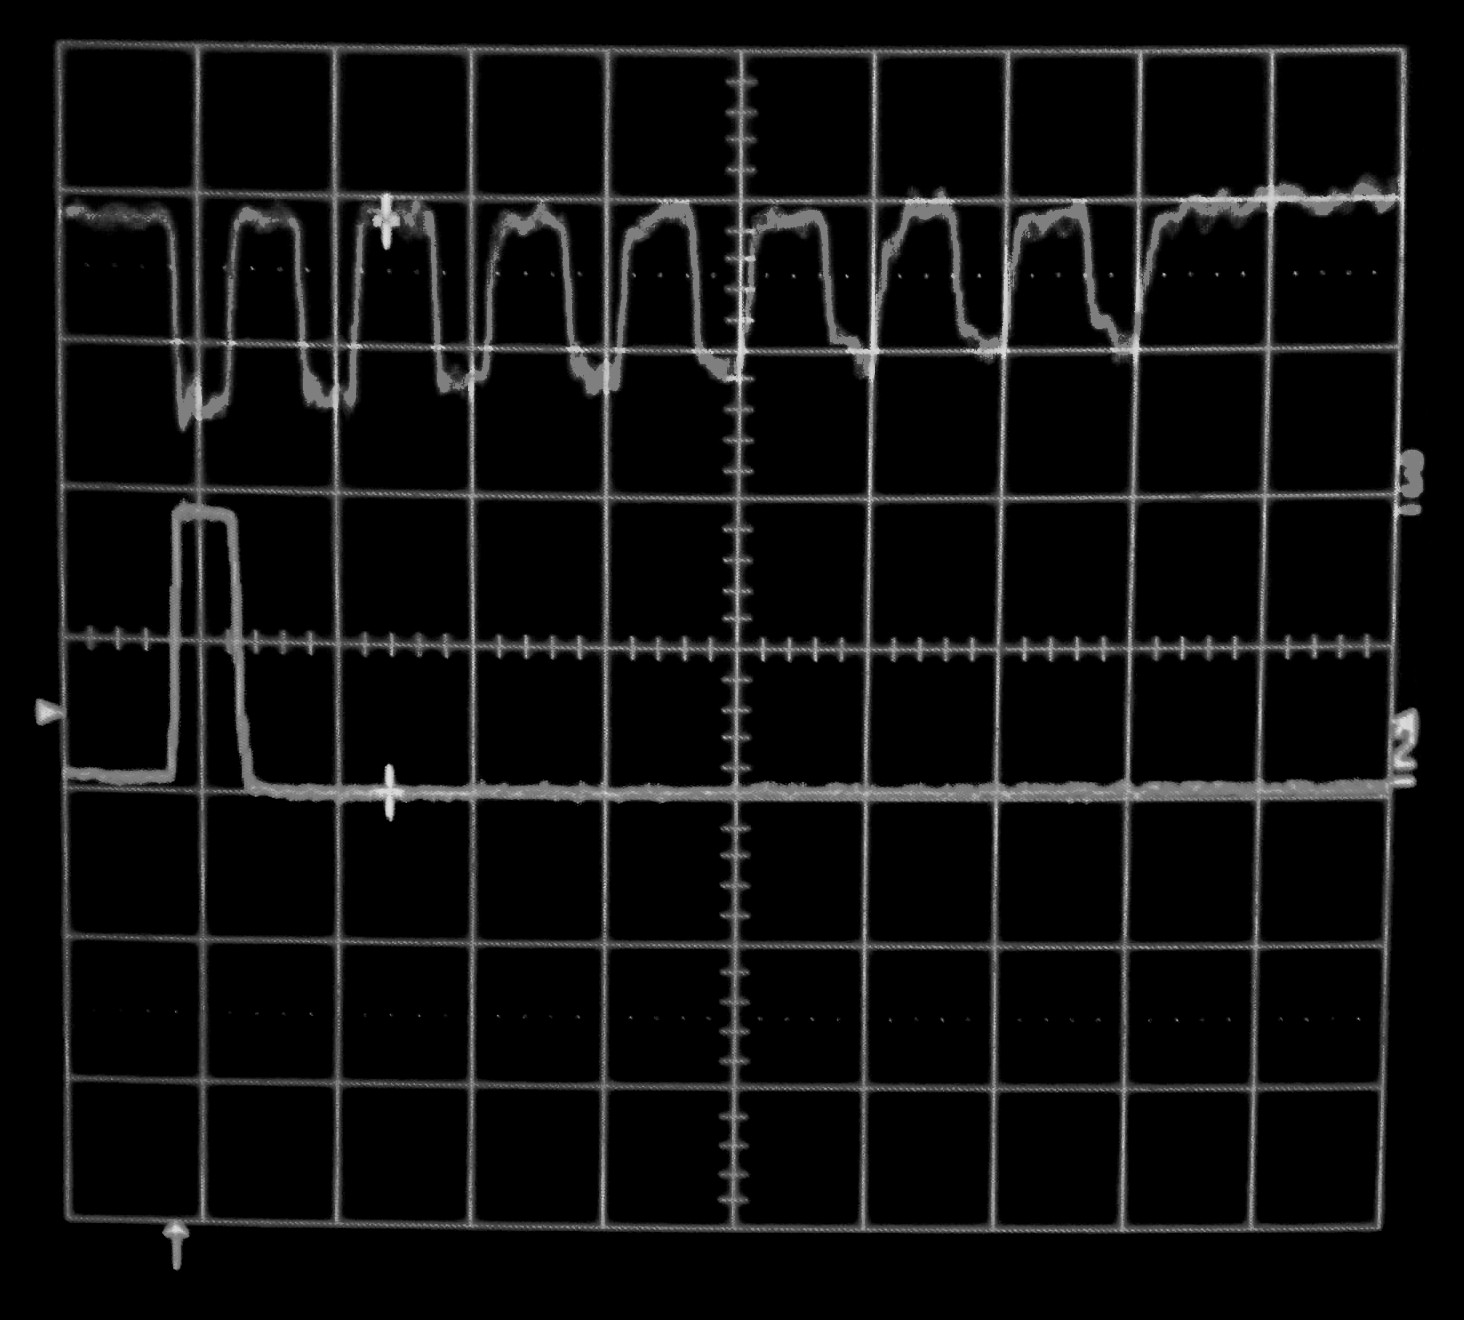
\includegraphics[height=2in, keepaspectratio=true]{graphics/delaypulse_bw.jpg}
	\caption{Oscilloscope capture from the output of a summer board. Eight channels are
		pulsed with a 12~mV synchronous pulse into the amplifier discriminator board. The amplified
		signals are routed through the delay lines into the summer board. The top trace is
		the output of the summer board. The bottom trace is the N-Hit sum output from the
		amplifier discriminator board, used as a trigger. The horizontal scale is 50~ns per division,
		the vertical scale is 100~mV per division. This figure illustrates the attenuation caused by the delay
		lines which will need to be compensated for in software. The first pulse shows an amplitude of approx 120~mV which would be expected with a gain of 10 from the system.
\label{fig:multipulse}}
\end{center}
\end{figure}

\subsection{Summer board}
\label{sec:Sum}
%
The summer board sums the analog channels after they have been delayed
and also sums the N-Hit sums from each of the 6 boards to make an
instantaneous N-Hit sum across the veto. 

The summer board has 8 inputs which are female SMA connectors. Each of
these inputs is fed, DC coupled, into a CFA to provide buffering. This
also provides the opportunity to fine tune the gain and equalize the
signals after the cable delay by adjusting the two feedback resistors.
The outputs are fed into another CFA configured as an analog summing
node. This outputs through a series resistor to an female MCX
connector. A short jumper cable connects the summer board output to
the digitizer input.  

Like the amplifier discriminator board, the summer board has local
power regulation.  Each board has one +5~V supply and one -5~V supply.
The regulators are fed by a common bipolar supply nominally at
$\pm$9~V.  The nominal values for current draw are 250~mA on the
positive rail and 250~mA on the negative rail.  A photo of the summer
board is shown in Figure~\ref{fig:boards}, an example test pulse in
through the summer board is shown in Figure~\ref{fig:summerpulse}.

\begin{figure}[ht]
	\begin{center}
		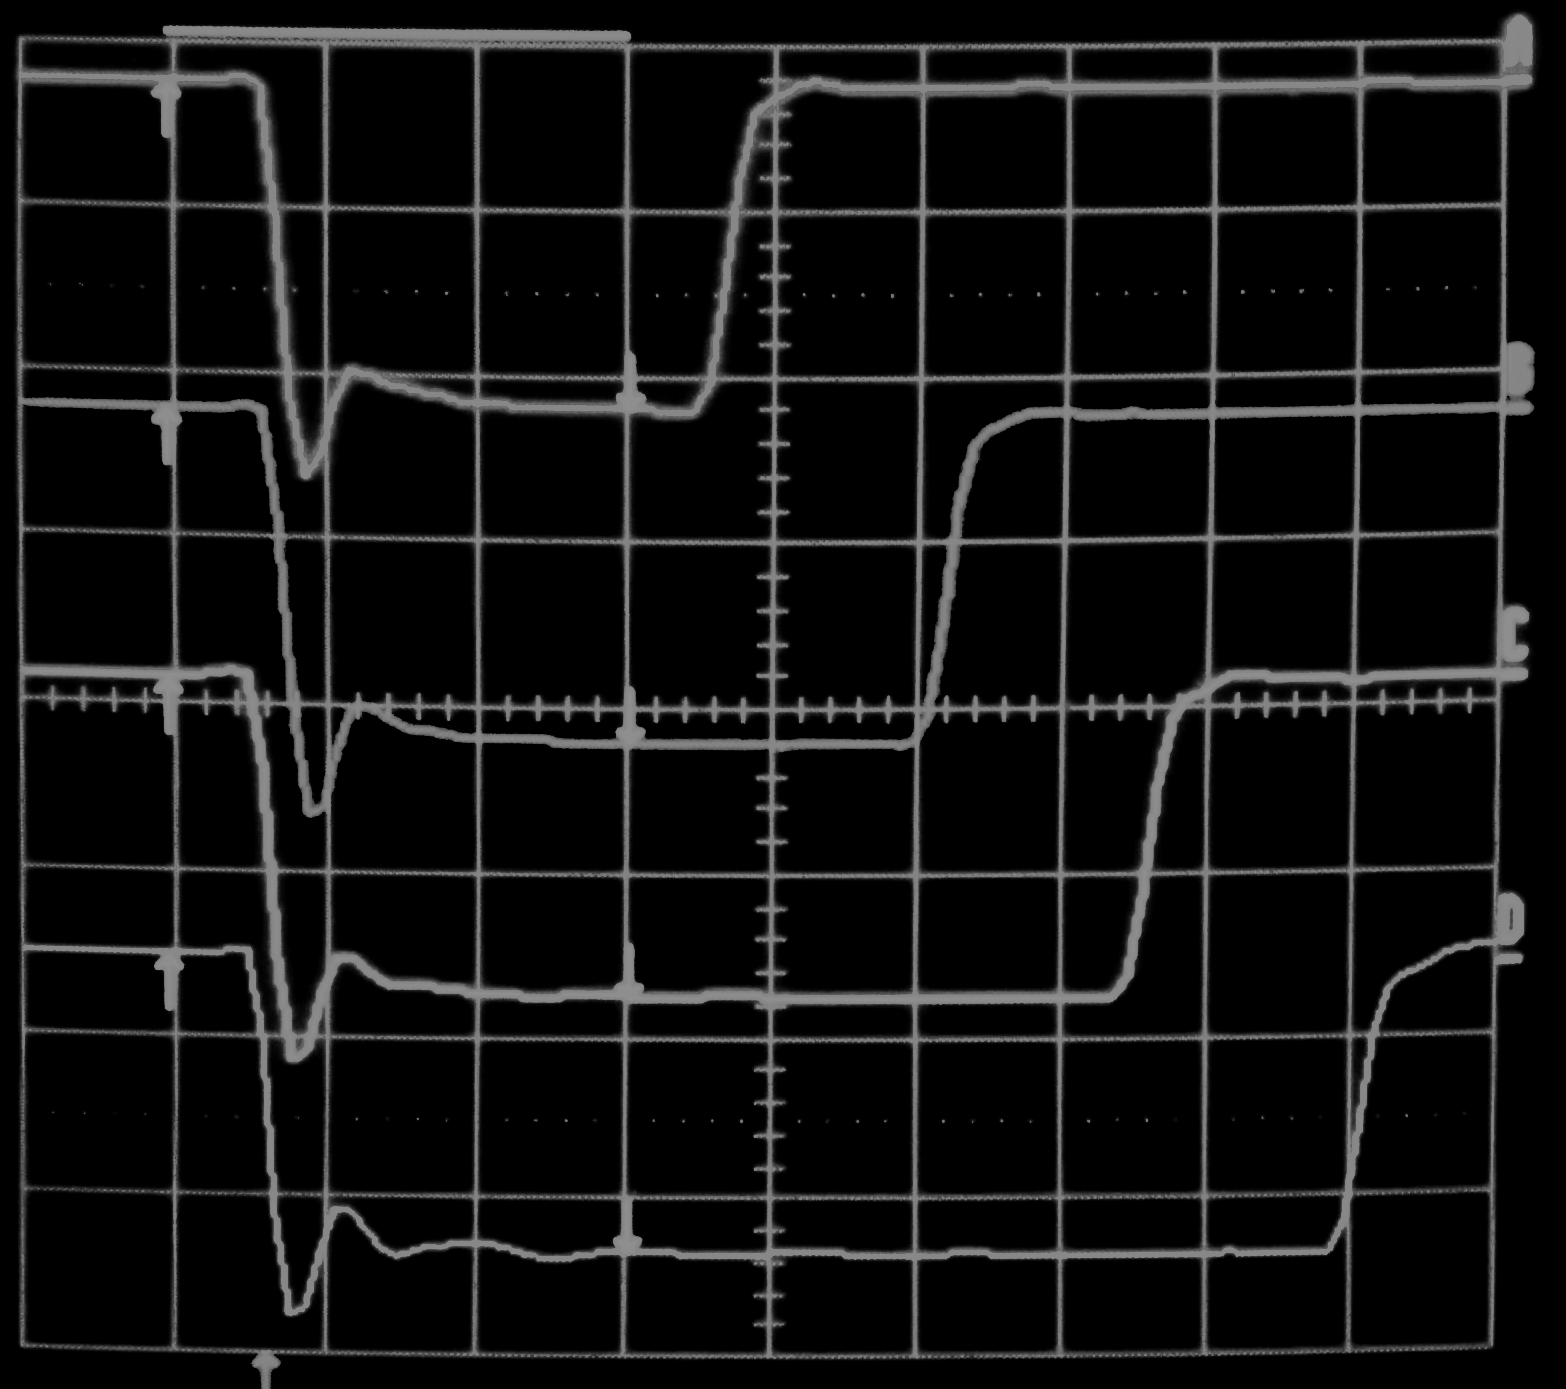
\includegraphics[height=2in, keepaspectratio=true]{graphics/sumpulseinput_bw.png}
		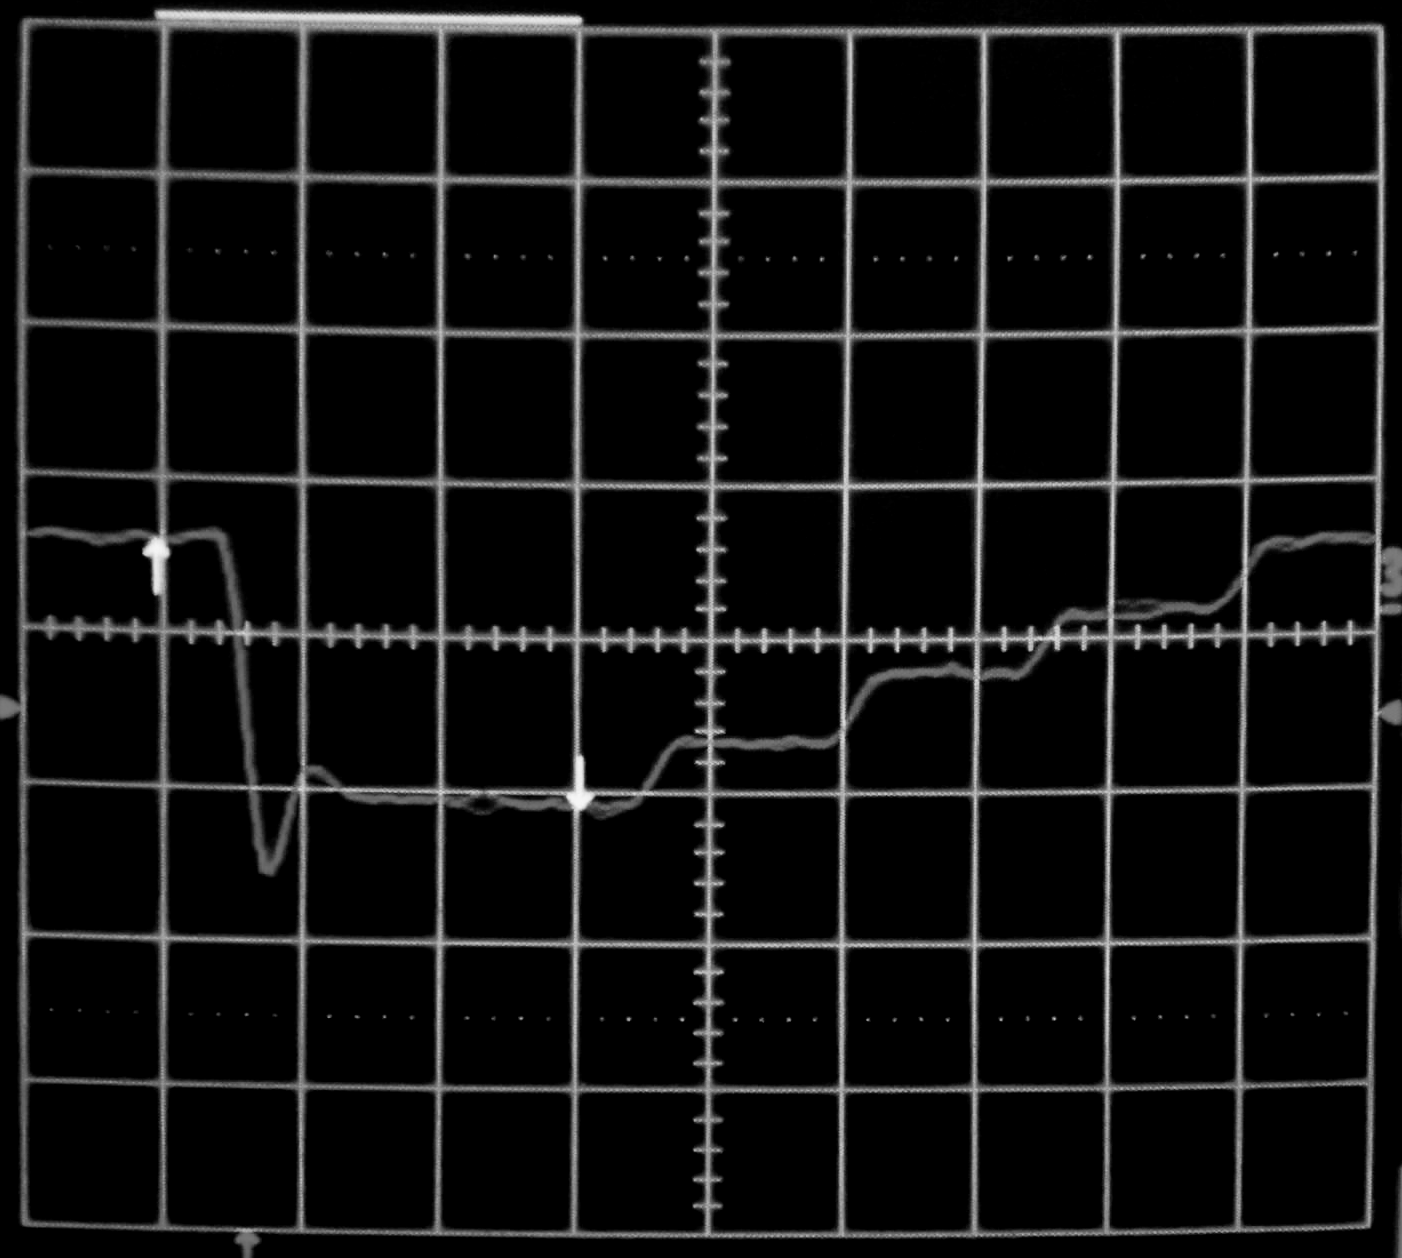
\includegraphics[height=2in, keepaspectratio=true]{graphics/sumpulseoutput_bw.png}
		\caption{Four input signals (left) and the output signal (right) of a summer board measured with a test pulse generator. The other four input channels are grounded. The horizontal scale is 10~ns per division, the vertical scale is 100~mV per division.  The active input channels have an amplitude of approximately 200~mV as shown in the left plot.  The summer outputs the sum attenuated by a factor of 5 as shown in the right plot.
		\label{fig:summerpulse}}
	\end{center}
\end{figure}

\begin{figure}[ht]
\begin{center}
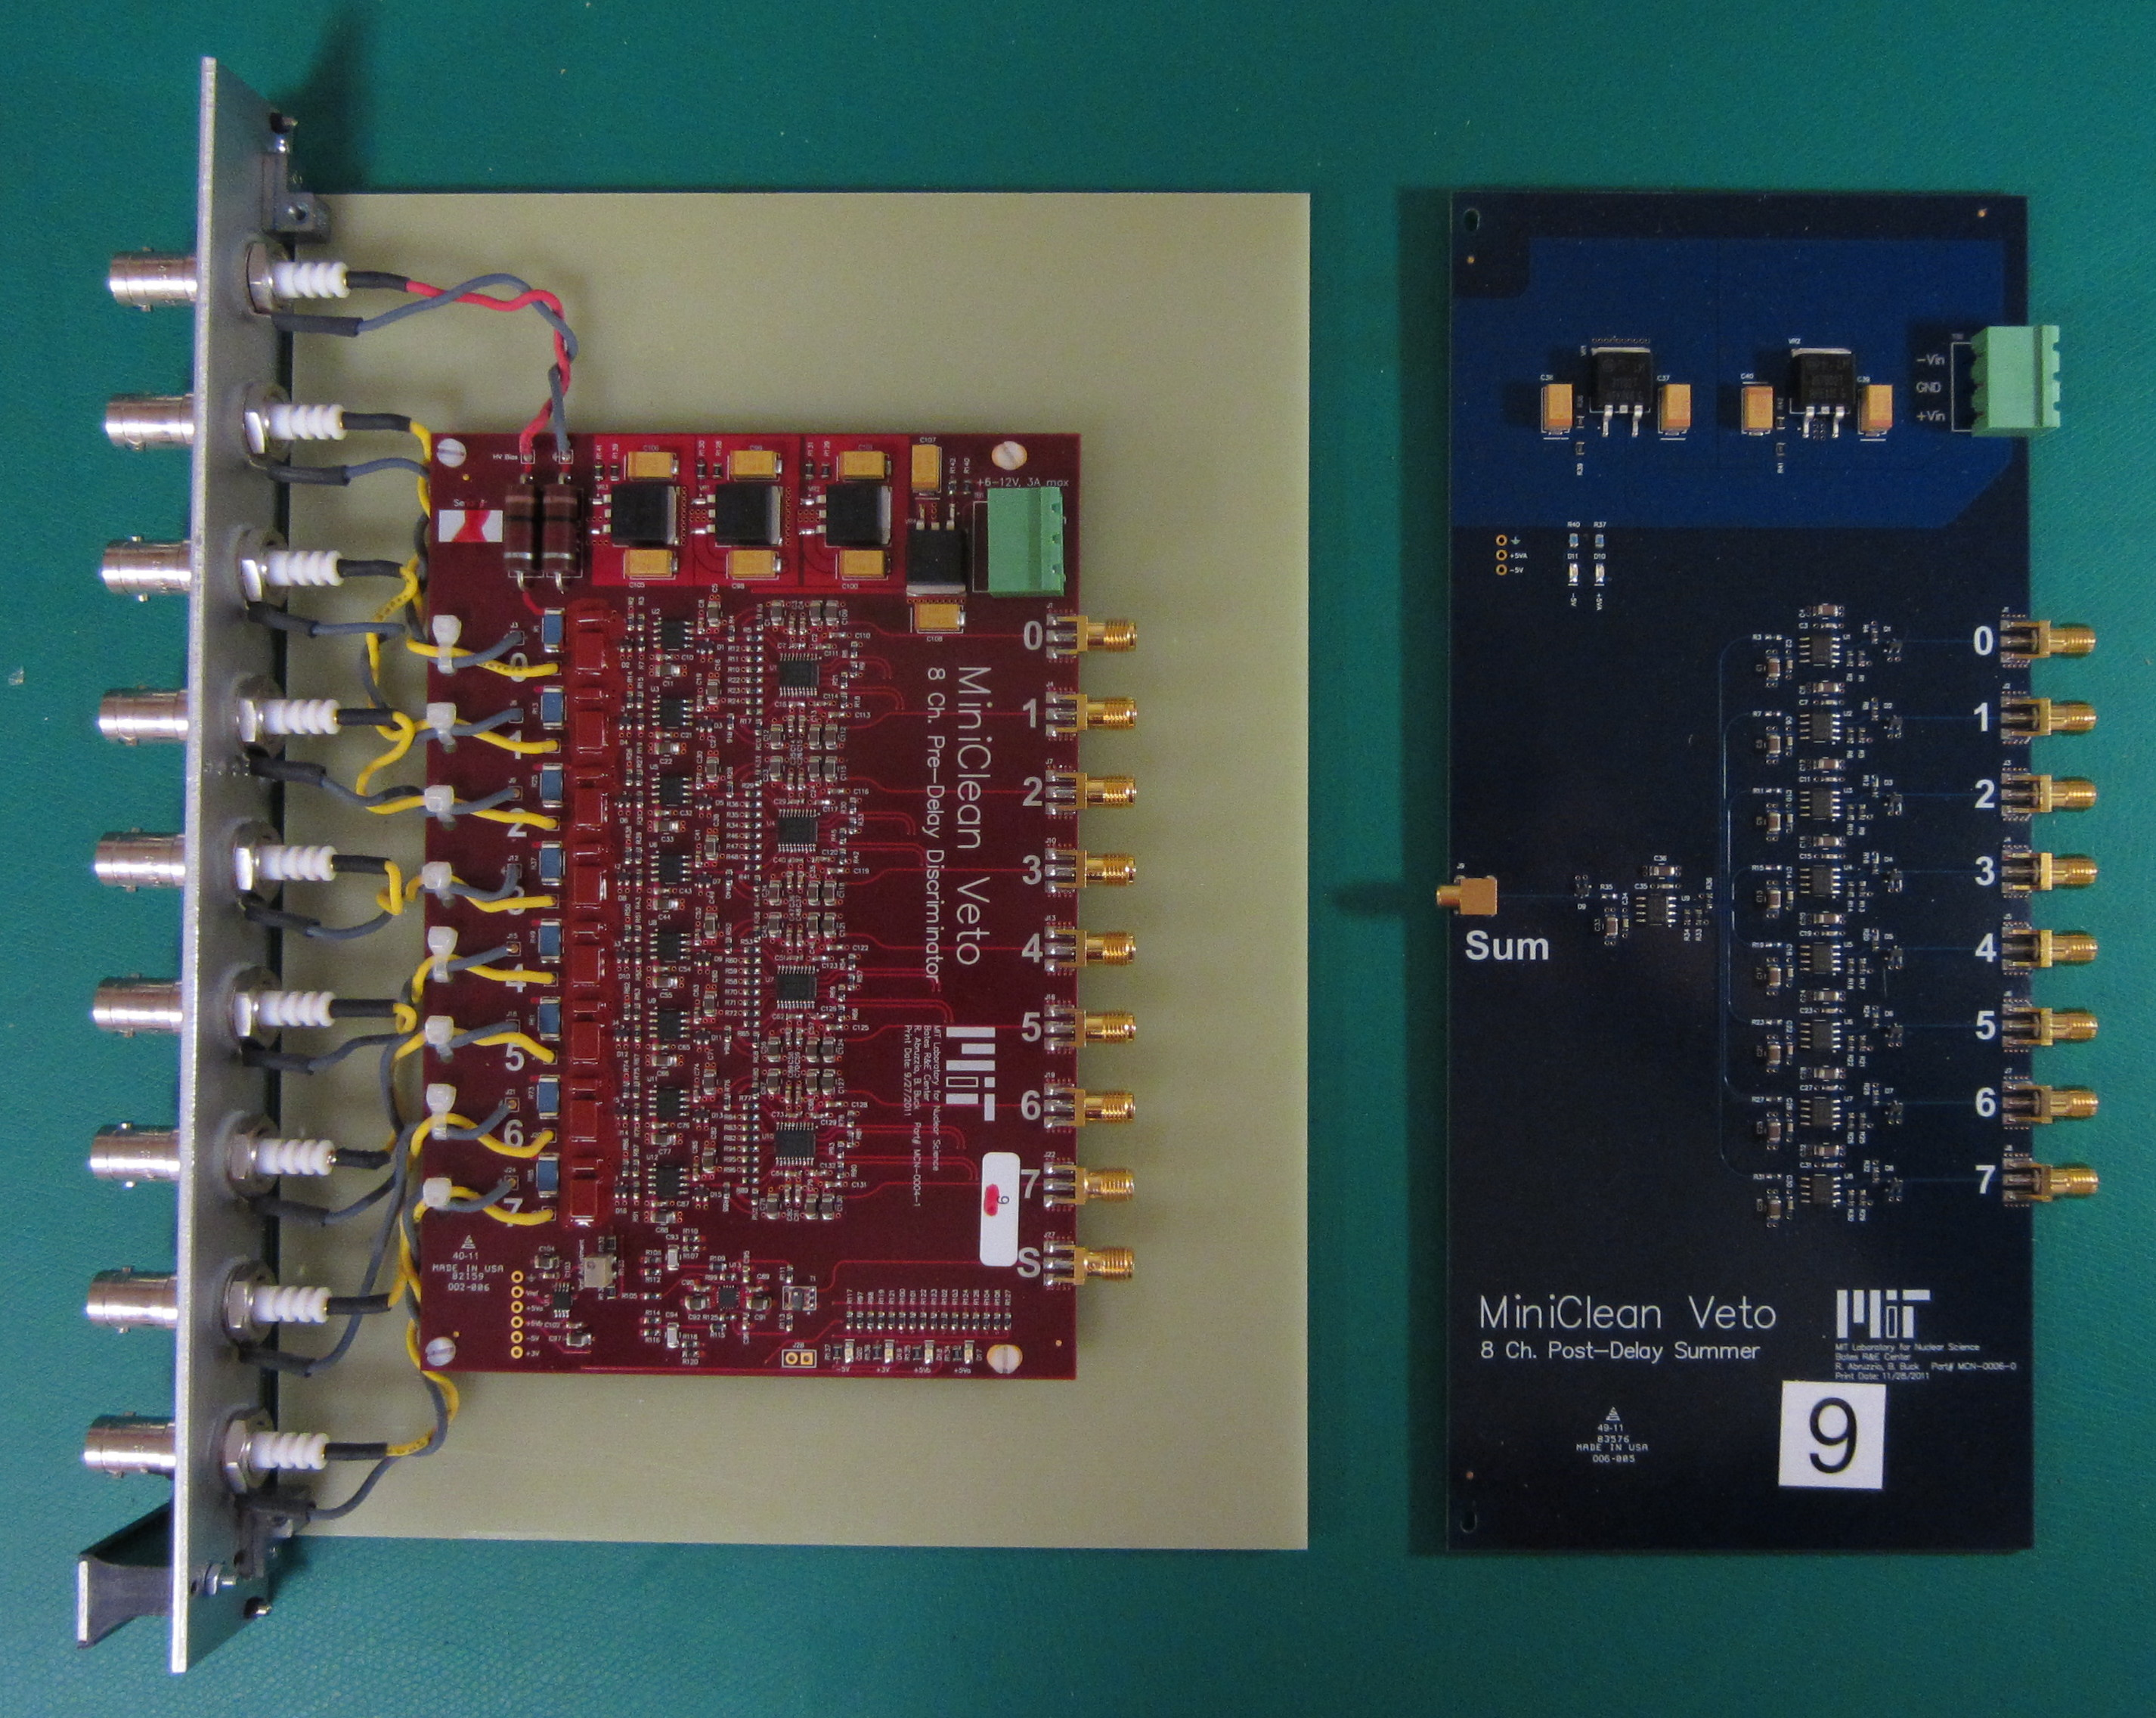
\includegraphics[width=4in, keepaspectratio=true]{graphics/boards.JPG}
\caption{Amplifier discriminator board (left) and summer board (right).
\label{fig:boards}}
\end{center}
\end{figure}

\subsection{Housing and assembly}
\label{sec:Housing}
%
The electronics are housed in a rack which holds a crate for the
electronics, a fan unit for cooling, a power supply unit, and all of
the delay lines. The power supply module provides $\pm$9~V up to
130~W. Estimated total power draw is 72~W. The power supply uses two
discrete 9~V switching power supplies which provide +9~V, 0~V, and
-9~V power rails running on the back of the rack. Connectors are
attached to these rails and insert into each of the electronics
boards. Each of the components was tested individually at MIT.
Amplifier discriminator boards were high-pot tested and all channels
were tested to ensure uniformity. Summer boards were similarly tested.
The boards were assembled into a VME style crate and mounted in a rack
together with the power supply unit, a fan unit, and the delay lines.
An integration test was done with the MiniCLEAN electronics at Boston
University to demonstrate the system running while attached to the
CAEN DAQ system.

\section{Summary}
\label{Summary}
%
An active muon veto detector has been designed, simulated, built, and
tested for the MiniCLEAN experiment.  The PMT and cable assemblies
have been tested to verify the single p.e. characteristics, the
operating voltages, and water-tight operation in similar conditions to
the MiniCLEAN veto tank.  A mechanical integration test was
successfully performed, verifying the hardware integrity and assembly
procedure.  A full test of the electronics chain using simulated
signals, integrated with the MiniCLEAN DAQ, demonstrated the veto
system electronics working properly. We were able to observe the N-Hit
trigger signal increase proportionally to the number of PMTs which
were hit, in the full electronics and DAQ system operated with
simulated pulse input. We also observed the correct output signals on
the time multiplexed outputs from the summer boards
(Figure~\ref{fig:multipulse}).  When operational on site at SNOLAB,
the full system will multiplex 48 PMT signals into 6 digitizer
channels and provide a system wide instantaneous N-Hit sum. The system
wide N-Hit will provide the veto trigger to the MiniCLEAN DAQ. The
system is now at SNOLAB ready for implementation in the experiment.

\acknowledgements
The authors would like to acknowledge support from NSF grant PHY-0970047 and the MIT Bates Research and Engineering Center.


\begin{thebibliography}{999}

\bibitem{ref:miniclean_physics} 
M. Ronquest, \emph{The MiniCLEAN single-phase noble liquid dark matter experiment}, IEEE Nucl.Sci.Symp.Conf.Rec. (2010) 1866-1872 \\

\bibitem{ref:sno_muon_flux} 
B. Aharmim {\it et al.}, \emph{Measurement of the cosmic ray and neutrino-induced muon flux at the Sudbury Neutrino Observatory}, Phys. Rev. D80 (2009) 012001 \\

\bibitem{ref:mei_and_hime} 
D. Mei and A. Hime, \emph{Muon-induced background study for underground laboratories}, Phys. Rev. D73 (2006) 053004

\bibitem{ref:geant4} 
J. Allison {\it et al.} \emph{Geant4 developments and applications}, IEEE Transactions on Nuclear Science 53 No. 1 (2006) 270-278 \\

\bibitem{ref:sno_pmt_paper}
C.J. Jillings {\it et al.} \emph{The Photomultiplier Tube Testing Facility for the Sudbury Neutrino Observatory}, Nucl. Instr. and Meth. A373 (1996) 421 \\

\bibitem{ref:gastler_thesis} 
	D. E. Gastler, \emph{Design of single phase liquid argon detectors for dark matter searches}, Boston University Ph.D. Thesis (2012) \\

\end{thebibliography}


\end{document}
